% Options for packages loaded elsewhere
\PassOptionsToPackage{unicode}{hyperref}
\PassOptionsToPackage{hyphens}{url}
%
\documentclass[
  man,floatsintext]{apa6}
\usepackage{amsmath,amssymb}
\usepackage{iftex}
\ifPDFTeX
  \usepackage[T1]{fontenc}
  \usepackage[utf8]{inputenc}
  \usepackage{textcomp} % provide euro and other symbols
\else % if luatex or xetex
  \usepackage{unicode-math} % this also loads fontspec
  \defaultfontfeatures{Scale=MatchLowercase}
  \defaultfontfeatures[\rmfamily]{Ligatures=TeX,Scale=1}
\fi
\usepackage{lmodern}
\ifPDFTeX\else
  % xetex/luatex font selection
\fi
% Use upquote if available, for straight quotes in verbatim environments
\IfFileExists{upquote.sty}{\usepackage{upquote}}{}
\IfFileExists{microtype.sty}{% use microtype if available
  \usepackage[]{microtype}
  \UseMicrotypeSet[protrusion]{basicmath} % disable protrusion for tt fonts
}{}
\makeatletter
\@ifundefined{KOMAClassName}{% if non-KOMA class
  \IfFileExists{parskip.sty}{%
    \usepackage{parskip}
  }{% else
    \setlength{\parindent}{0pt}
    \setlength{\parskip}{6pt plus 2pt minus 1pt}}
}{% if KOMA class
  \KOMAoptions{parskip=half}}
\makeatother
\usepackage{xcolor}
\usepackage{graphicx}
\makeatletter
\newsavebox\pandoc@box
\newcommand*\pandocbounded[1]{% scales image to fit in text height/width
  \sbox\pandoc@box{#1}%
  \Gscale@div\@tempa{\textheight}{\dimexpr\ht\pandoc@box+\dp\pandoc@box\relax}%
  \Gscale@div\@tempb{\linewidth}{\wd\pandoc@box}%
  \ifdim\@tempb\p@<\@tempa\p@\let\@tempa\@tempb\fi% select the smaller of both
  \ifdim\@tempa\p@<\p@\scalebox{\@tempa}{\usebox\pandoc@box}%
  \else\usebox{\pandoc@box}%
  \fi%
}
% Set default figure placement to htbp
\def\fps@figure{htbp}
\makeatother
\setlength{\emergencystretch}{3em} % prevent overfull lines
\providecommand{\tightlist}{%
  \setlength{\itemsep}{0pt}\setlength{\parskip}{0pt}}
\setcounter{secnumdepth}{-\maxdimen} % remove section numbering
% Make \paragraph and \subparagraph free-standing
\makeatletter
\ifx\paragraph\undefined\else
  \let\oldparagraph\paragraph
  \renewcommand{\paragraph}{
    \@ifstar
      \xxxParagraphStar
      \xxxParagraphNoStar
  }
  \newcommand{\xxxParagraphStar}[1]{\oldparagraph*{#1}\mbox{}}
  \newcommand{\xxxParagraphNoStar}[1]{\oldparagraph{#1}\mbox{}}
\fi
\ifx\subparagraph\undefined\else
  \let\oldsubparagraph\subparagraph
  \renewcommand{\subparagraph}{
    \@ifstar
      \xxxSubParagraphStar
      \xxxSubParagraphNoStar
  }
  \newcommand{\xxxSubParagraphStar}[1]{\oldsubparagraph*{#1}\mbox{}}
  \newcommand{\xxxSubParagraphNoStar}[1]{\oldsubparagraph{#1}\mbox{}}
\fi
\makeatother
% definitions for citeproc citations
\NewDocumentCommand\citeproctext{}{}
\NewDocumentCommand\citeproc{mm}{%
  \begingroup\def\citeproctext{#2}\cite{#1}\endgroup}
\makeatletter
 % allow citations to break across lines
 \let\@cite@ofmt\@firstofone
 % avoid brackets around text for \cite:
 \def\@biblabel#1{}
 \def\@cite#1#2{{#1\if@tempswa , #2\fi}}
\makeatother
\newlength{\cslhangindent}
\setlength{\cslhangindent}{1.5em}
\newlength{\csllabelwidth}
\setlength{\csllabelwidth}{3em}
\newenvironment{CSLReferences}[2] % #1 hanging-indent, #2 entry-spacing
 {\begin{list}{}{%
  \setlength{\itemindent}{0pt}
  \setlength{\leftmargin}{0pt}
  \setlength{\parsep}{0pt}
  % turn on hanging indent if param 1 is 1
  \ifodd #1
   \setlength{\leftmargin}{\cslhangindent}
   \setlength{\itemindent}{-1\cslhangindent}
  \fi
  % set entry spacing
  \setlength{\itemsep}{#2\baselineskip}}}
 {\end{list}}
\usepackage{calc}
\newcommand{\CSLBlock}[1]{\hfill\break\parbox[t]{\linewidth}{\strut\ignorespaces#1\strut}}
\newcommand{\CSLLeftMargin}[1]{\parbox[t]{\csllabelwidth}{\strut#1\strut}}
\newcommand{\CSLRightInline}[1]{\parbox[t]{\linewidth - \csllabelwidth}{\strut#1\strut}}
\newcommand{\CSLIndent}[1]{\hspace{\cslhangindent}#1}
\ifLuaTeX
\usepackage[bidi=basic]{babel}
\else
\usepackage[bidi=default]{babel}
\fi
\babelprovide[main,import]{english}
% get rid of language-specific shorthands (see #6817):
\let\LanguageShortHands\languageshorthands
\def\languageshorthands#1{}
\ifLuaTeX
  \usepackage[english]{selnolig} % disable illegal ligatures
\fi
% Manuscript styling
\usepackage{upgreek}
\captionsetup{font=singlespacing,justification=justified}

% Table formatting
\usepackage{longtable}
\usepackage{lscape}
% \usepackage[counterclockwise]{rotating}   % Landscape page setup for large tables
\usepackage{multirow}		% Table styling
\usepackage{tabularx}		% Control Column width
\usepackage[flushleft]{threeparttable}	% Allows for three part tables with a specified notes section
\usepackage{threeparttablex}            % Lets threeparttable work with longtable

% Create new environments so endfloat can handle them
% \newenvironment{ltable}
%   {\begin{landscape}\centering\begin{threeparttable}}
%   {\end{threeparttable}\end{landscape}}
\newenvironment{lltable}{\begin{landscape}\centering\begin{ThreePartTable}}{\end{ThreePartTable}\end{landscape}}

% Enables adjusting longtable caption width to table width
% Solution found at http://golatex.de/longtable-mit-caption-so-breit-wie-die-tabelle-t15767.html
\makeatletter
\newcommand\LastLTentrywidth{1em}
\newlength\longtablewidth
\setlength{\longtablewidth}{1in}
\newcommand{\getlongtablewidth}{\begingroup \ifcsname LT@\roman{LT@tables}\endcsname \global\longtablewidth=0pt \renewcommand{\LT@entry}[2]{\global\advance\longtablewidth by ##2\relax\gdef\LastLTentrywidth{##2}}\@nameuse{LT@\roman{LT@tables}} \fi \endgroup}

% \setlength{\parindent}{0.5in}
% \setlength{\parskip}{0pt plus 0pt minus 0pt}

% Overwrite redefinition of paragraph and subparagraph by the default LaTeX template
% See https://github.com/crsh/papaja/issues/292
\makeatletter
\renewcommand{\paragraph}{\@startsection{paragraph}{4}{\parindent}%
  {0\baselineskip \@plus 0.2ex \@minus 0.2ex}%
  {-1em}%
  {\normalfont\normalsize\bfseries\itshape\typesectitle}}

\renewcommand{\subparagraph}[1]{\@startsection{subparagraph}{5}{1em}%
  {0\baselineskip \@plus 0.2ex \@minus 0.2ex}%
  {-\z@\relax}%
  {\normalfont\normalsize\itshape\hspace{\parindent}{#1}\textit{\addperi}}{\relax}}
\makeatother

\makeatletter
\usepackage{etoolbox}
\patchcmd{\maketitle}
  {\section{\normalfont\normalsize\abstractname}}
  {\section*{\normalfont\normalsize\abstractname}}
  {}{\typeout{Failed to patch abstract.}}
\patchcmd{\maketitle}
  {\section{\protect\normalfont{\@title}}}
  {\section*{\protect\normalfont{\@title}}}
  {}{\typeout{Failed to patch title.}}
\makeatother

\usepackage{xpatch}
\makeatletter
\xapptocmd\appendix
  {\xapptocmd\section
    {\addcontentsline{toc}{section}{\appendixname\ifoneappendix\else~\theappendix\fi: #1}}
    {}{\InnerPatchFailed}%
  }
{}{\PatchFailed}
\makeatother
\keywords{politics, morality, psycholinguistics}
\usepackage{csquotes}
\usepackage{bookmark}
\IfFileExists{xurl.sty}{\usepackage{xurl}}{} % add URL line breaks if available
\urlstyle{same}
\hypersetup{
  pdftitle={Moral Foundations of U.S. Political News Organizations},
  pdfauthor={William E. Padfield1, Erin M. Buchanan, Ph.D.2, \& Kayden N. Jordan, Ph.D.2},
  pdflang={en-EN},
  pdfkeywords={politics, morality, psycholinguistics},
  hidelinks,
  pdfcreator={LaTeX via pandoc}}

\title{Moral Foundations of U.S. Political News Organizations}
\author{William E. Padfield\textsuperscript{1}, Erin M. Buchanan, Ph.D.\textsuperscript{2}, \& Kayden N. Jordan, Ph.D.\textsuperscript{2}}
\date{}


\shorttitle{MORAL NEWS}

\authornote{

William Padfield completed this project as part of his thesis requirements for a master's degree candidate in Psychology at Missouri State University. Submitted to Meta-Psychology. Participate in open peer review by commenting through hypothes.is directly on this preprint. The full editorial process of all articles under review at Meta-Psychology can be found following this link: \url{https://tinyurl.com/mp-submissions}

Correspondence concerning this article should be addressed to William E. Padfield, 901 S. National Ave, Springfield, MO, 65897. E-mail: \href{mailto:wpadfield@gmail.com}{\nolinkurl{wpadfield@gmail.com}}

}

\affiliation{\vspace{0.5cm}\textsuperscript{1} Missouri State University\\\textsuperscript{2} Harrisburg University of Science and Technology}

\abstract{%
Partisan differences and diviseness have become an increasing hot topic in psychological research. Many theories have been proposed to explain these differences and divisions including Moral Foundations Theory. The current research seeks determine if a linguistic measure of Moral Foundations, the Moral Foundations Dictionary (MFD) can unveil these theoretical partisan differences. In Study 1, we explored the MFD-Moral Foundations Questionnaire's measurement overlap using a multi-trait multi-method model and determined if current predictive shortcomings of the MFD can be improved with additional linguistic content. Next, we examined two replication extensions of previous work assessing the differences in political articles on moral differences using the MFD. Through web scraping, we extracted articles from popular partisan news sources' websites, calculated MFD word frequencies, and identified words' respective valences. This process attempts to uncover news outlets' positive or negative endorsements of certain moral dimensions concomitant with a particular ideology. In Study 2, we gathered political articles from four sources. In Study 3, we expanded their number of sources to 10 and analyzed articles that pertain to two specific topics: the 2018 confirmation hearings of U.S. Supreme Court Justice Brett Kavanaugh and the partial U.S. Government Shutdown of 2018-2019. Results from all studies indicate that the MFD may not consistently show exptected partisan differences, shedding doubt on the usefulness of the MFD.
}



\begin{document}
\maketitle

The field of moral psychology has a long history with modern moral
psychology beginning in the late 1960s with Lawrence Kohlberg's theory
of moral development (Kohlberg \& Hersh, 1977). Since then, Kohlberg's theory has
been highly criticized with numerous theories and hypotheses proposed to
replace it. One of these theories is Moral Foundations Theory (MFT)
proposed by Haidt and colleagues (Haidt \& Graham, 2007; Haidt \& Joseph, 2004). While the
theory itself has been widely criticized and debated, the goal of the
current work is to tackle a related measurement issue, the Moral
Foundations Dictionary (MFD, Graham, Haidt, \& Nosek, 2009). Graham et al. (2009) developed the
MFD - a lexicon-based linguistic measure of MFT - arguing that moral
concerns and the propositions of MFT could be measured and tested with
the words people use. Here we first review evidence and criticisms
against this assumption. We then provide our own test of the MFD using a statistical validity assessment and partisan news articles.

\subsection{Moral Foundations Measurement}\label{moral-foundations-measurement}

Haidt and Joseph (2004) and Haidt and Graham (2007)
formulated MFT as a method by which to capture the entirety of humans'
moral domain. They argued that older theories of moral psychology were
focused primarily on issues of justice, fairness, and caring, which are
individually focused foundations of morality that align with the beliefs
of political liberals. In other words, moral psychology ignored the
valid moral foundations of conservatives. MFT holds that people's moral
domain can be mapped by quantifying their endorsement of five moral
foundations: harm/care, fairness/reciprocity, ingroup/loyalty,
authority/respect, and purity/sanctity (Haidt \& Graham, 2007). Thus, they
proposed that the addition of these two additional domains could
adequately capture the broader spectrum of morality. Throughout the rest of the article, we will use the first word from each of these continuums to denote the foundation area.

Measurement of MFT has traditionally focused on two options: 1) the
Moral Foundations Questionnaire (MFQ) - a typical Likert-type survey
instrument that measures moral relevance of each foundation to an
individual and the moral judgment of various scenarios depicting each
foundation, and 2) the Moral Foundations Dictionary (MFD) which was
designed to capture language's role in moral reasoning and justification
as used in speech and text (Graham et al., 2009, 2011). The MFQ is a
30-item scale with 15 items on the moral relevance and judgment
scenarios. The 15 moral relevance items are equally divided among the
five foundations and examine how relevant a condition is to making a
moral judgment on a scale of 1 (\emph{not at all relevant}) to 6 (\emph{extremely
relevant}). These relevance items include examples such as: ``Whether or
not someone used violence (harm),'' ``Whether or not someone was denied
his or her rights (fairness),'' ``Whether or not someone showed a lack
of loyalty (ingroup),'' ``Whether or not an action caused chaos or
disorder (authority),'' and ``Whether or not someone did something
disgusting (purity).'' The moral judgments items are also equally
divided between the foundations and ask on a six-point scale how much
one agrees with each of the statements. These judgment items include:
``One of the worst things a person can do is hurt a defenseless animal
(harm),'' ``Justice is the most important requirement of a society
(fairness),'' ``I am proud of my country's history (ingroup),'' ``Men
and women each have different roles to play in society (authority),''
and ``Chastity is an important and valuable virtue (purity).''

The internal consistency of the MFQ from Graham et al. (2011) was \(\alpha\) = .73
averaged across subscales with a range of \(\alpha\) = .65-.84. Across six
studies, the MFQ was found to have an average Cronbach's alpha of .63
for harm, .64 for fairness, .56 for ingroup, .59 for authority,
and .71 for purity (Federico, Weber, Ergun, \& Hunt, 2013; Graham et al., 2009; Graham, Nosek, \& Haidt, 2012; Weber \& Federico, 2013). Test-retest reliability was \emph{r} = .68-.82 using a sample of
123 college students. Confirmatory factor analysis supported a
well-fitted five-factor model (harm, fairness,
ingroup, authority, and purity) over two,
individual (harm and fairness) versus group (ingroup, authority,
and purity) foundations, or three, autonomy (harm, fairness),
community (ingroup, authority), and divinity (purity) ethics,
foundations factor model. The five-factor structure also fit for
non-Western samples, thus, providing evidence of the MFQ
generalizability. Convergent validity was supported with correlations on
other measures of morality (Graham et al., 2011).

The MFD is composed of 259 words, with around 50 words assigned to each
of the five foundations. Graham et al. (2009) created a preliminary list of words
that they believed would be associated with the five foundations. Words
such as \emph{war} and \emph{peace} should indicate a greater concern with harm
foundation whereas words such as \emph{homeland} and \emph{terrorism} should
indicate a greater concern with the ingroup foundation. The other
foundation dictionaries include \emph{equal} and \emph{justice} (fairness),
\emph{honor} and \emph{protest} (authority), and \emph{holy} and \emph{sin} (purity). To
validate the word sets, Graham et al. (2009) examined the frequency of MFD words
in liberal and conservative sermons using the Linguistic Inquiry and
Word Count (LIWC, Pennebaker, Booth, \& Frances, 2007) computer program. They found liberal
ministers used harm, fairness, and ingroup words more often than
conservative ministers who used authority and purity words more
often. Although conservative ministers were expected to use more
ingroup words based on political ideology and previous research, an
examination of the way liberal ministers used ingroup words revealed a
tendency for the use of ingroup words to glorify rebellion and promote
independence (i.e., the opposite direction from ingroup definitions).
Effect sizes indicated relatively sizable difference between liberal and
conservative sermons with Cohen's \(d_s\) values ranging from 0.56 to 1.27.

In contrast to this approach, Sagi and Dehghani (2014) explored how moral words were
used paired with other co-occurring concepts using Latent Semantic
Analysis (LSA). They examined three different moral issues in different
contexts to piece out specific moral words and their collocates. First,
they looked at how moral words were used in relation to the World Trade
Center compared to the Empire State Building in the New York Times from
1987-2007. After 9-11, the number of moral words associated with the
World Trade Center increased, specifically harm words from the MFD.
Second, they considered the changes in how moral words were paired with
mosque used in blogs as a response to the debate of building a mosque
near Ground Zero following 9-11. They found words from the MFD were used
more often with mosque during the main debate and then the co-occurrence
decreased afterwards. Lastly, they examined moral language tied to the
abortion debate in Congress. Republicans used more moral language
overall; more specifically, Republicans tended to use more words
associated with the purity foundation; while Democrats used more words
associated with the fairness foundation.

\subsection{Critiques of Moral Foundations}\label{critiques-of-moral-foundations}

MFT has received criticism on the grounds that its assumptions regarding
moral intuitions have little empirical basis. Suhler, Churchland, and Joseph (2011) criticized the
content and taxonomy of the five foundations and question whether or not
the foundations are sufficiently distinct as to stand as their own
foundation. Likewise, Gray and Keeney (2015) argued that the measurement of the moral
foundations confounds morality with other constructs (such as weirdness)
and that the moral foundations lack statistical and conceptual distinction.
Schein and Gray (2015) argued that harm-based morality is the most parsimonious and
logical explanation for MFT findings.

Beyond the critiques of the theory itself, many have also provided
strong critiques of the measurement using MFD. Conducting two close
conceptual replication studies using religious sermons and six extension
studies using U.S. Congressional speeches, party platforms, State of the
Union addresses, media outlets, and political organization texts,
Frimer (2020) found that the liberal-conservative differences found in the
original study replicated in only 30\% of cases and the effect sizes were
over 30 times smaller than reported in Graham et al. (2009). In a meta-analysis,
the theorized differences were only found for authority and purity
(e.g., conservatives used more authority and purity words). Loyalty was
contrary to theoretical predictions (e.g., used more by liberals), and
no differences were found for harm and fairness. Additionally,
Frimer (2020) tested the theory under the most forgiving conditions using
not only the original MFD but also the revised MFD2 as well using log
transformed scores and raw scores. Even under the best circumstances
(log transformed MFD2 scores), only two of the foundations showed
theorized differences but with very small effects.

Other studies have
also found conflicting findings which fail to support the basic
assertions of MFT. Exploring the political Twitterverse, Sterling and Jost (2018)
found differences in the MFD depend on political sophistication. For
example, harm words were used more by liberals only if they had low
levels of political sophistication; at high levels of political
sophistication, conservatives used more harm words. While the MFD has
not been extensively used (at least in published research), studies
which have use the MFD to test partisan differences have found mixed
results in terms of supporting MFT (Clifford \& Jerit, 2013; Frimer, Tell, \& Haidt, 2015; Sagi \& Dehghani, 2014). Like Frimer (2020), we attempt to give the MFD the best chance
for success by both increasing linguistic content and incorporating a weighting method to address the
skewedness and sparsity of the linguistic data.

The most successful attempts to validate a linguistic measure of moral
foundations have used more complex methods (compared to the original
dictionary-based approach). These attempts generally fall into two
categories: human annotations and semantic representations. Hopp, Fisher, Cornell, Huskey, and Weber (2021)
assessed the first approach where instead of relying on `experts', a
large sample of lay people were crowdsourced to manually annotate
document for content relevant to each foundation. While
resource-intensive, this method better captures how people may encounter
and judge moral issues in everyday life leading to a more ecologically
valid dictionary. Garten, Boghrati, Hoover, Johnson, and Dehghani (2016) examined the second category which
instead relies on data-driven semantic analysis. Using shallow neural
net models like word2vec (Mikolov, Chen, Corrado, \& Dean, 2013), moral foundations
were measured using semantic similarity vectors rather than simple word
counts. Here, we try to augment the simpler approach to add more context
to see if the MFD liberal-conservative differences can be replicated.

First, we use the MFQ and MFD in a multi-trait multi-method approach to
determine if the dictionary can be improved and mapped into the
theoretical MFT traits. This study examined the measurement overlap
between these two sources, as well as the latent traits after
controlling for method-related measurement. Using the results from this study, we
examined two conceptual replications of Frimer (2020). We test the
liberal-conservative difference proposed by MFT using partisan media
content and the MFD. We first test differences in a general news corpus
compared liberal sources (National Public Radio {[}NPR{]} and the New York
Times {[}NYT{]}) to conservative sources (Fox News and Breitbart). Second,
we examined news about specific political events: Brett Kavanaugh's U.S.
Supreme Court nomination and the U.S. Government Shutdown in 2018-2019.
In the second study, the news sources were expanded to cover NYT, NPR,
Slate, Huffington Post, and Politico on the liberal side and Fox News,
Breitbart, The Rush Limbaugh Show, The Blaze, and Sean Hannity on the
conservative side. To address potential issues of measurement with the
MFD, the MFD was combined with the information produced in Study 1 and
weighted by valence to create weighted percentages to better specify
endorsement. Like Frimer (2020), results were judged based on the
direction of the liberal-conservative difference compared MFT
predictions and the size of the effect compared to past studies.

\section{Study 1}\label{study-1}

We approached this study with the intention to answer a method question.
That is, this portion of the current research was conducted in order to
solidify the best method by which to analyze political news text under
the MFT framework while also alleviating some of the aforementioned
potential dictionary issues with the MFD. In this set of studies, we
examined the MFD and MFQ within the same study. The first two
sub-studies were used to develop a (potentially) larger dictionary for
the MFD and collect data on both scales. The original dictionary was
developed conceptually, identifying words that \emph{should} go with each
moral trait. In Study 1.1 and 1.2, we collect data to expand the
dictionary. The last sub-study examined the MFD and MFQ using
multi-trait multi-method (MTMM) analysis using guidelines from
Byrne (2001) and Widaman (1985).

\subsection{Study 1.1}\label{study-1.1}

In this study, participants were given a word association task elicit
additional semantically related word forms for each moral foundation.
This data was used to expand the MFD for each latent area to determine
if these additional words could improve scores and test measurement
relation to the MFQ in Study 1.3.

\subsubsection{Participants}\label{participants}

466 participants were assessed from a large Midwestern
university. Participants were given course credit for their introductory
psychology course for completing the study. 14
participants had missing data on the MFQ and were excluded from
analyses. The MFQ data was screened for multivariate outliers with
Mahalanobis distance as described in Tabachnick and Fidell (2012), and
15 outliers were found using
\(\chi^2_{p < .001}\)(15) = 37.70. These participants
were excluded from further analyses, representing 437
final participants. Participants were asked to denote their political
party, and 25.9\%
indicated they were Democrats,
42.8\% were
Republican, and
31.1\% indicated
they were Independent. 0.2\%
of values were missing for this question.

\subsubsection{Materials and Procedure}\label{materials-and-procedure}

A complete example of the survey can be found online at
\url{https://osf.io/6mv2g}. First, participants were given a description of
associative memory as the relation between words that comes about
through many pairings in writing and speech. Next, the free association
task, similar to that used in Nelson, McEvoy, and Schreiber (2004) and De Deyne, Navarro, Perfors, Brysbaert, and Storms (2019) was described
to the participants as listing the ``first word that pops into mind''. The
participants were then given three example free association cues,
\emph{lost}, \emph{old}, and \emph{article}. For each cue, participants were asked to
write all the words that come to mind. To elicit free association to the
moral foundation areas, participants were given the following
instructions:

``Moral Foundations Theory states that when making moral
judgments/decisions, the concerns people have can be divided into five
categories. Below are labels of each of these five categories. You will
then be asked to list words you think are associated with each of the
labels.''

Each of the foundation pairs were listed together (i.e., harm,
fairness, etc.) with a space for participants to list
their free association concepts. After the free association task,
participants were then given the 15-items from the moral relevance
section of the MFQ as described in the introduction. Last, participants
were asked to denote their political orientation from 1 \emph{conservative}
to 10 \emph{liberal}, as well as which political party they associated with:
Democrat, Republican, and Independent. The survey was delivered through
Qualtrics, and participants were recruited through the online
participant management system for the university (SONA). Each
participant signed an online consent form at the beginning of the study
and was given participation credit at the end of the study.

\subsubsection{Results}\label{results}

All data was screening for inaccurate responses, as well as missing
data, as described in the participant section. The final MFQ data was
screened for assumptions of normality, linearity, and homoscedasticity.
The MFQ data was slightly skewed but otherwise linear and homoscedastic
after accounting for skew. No transform was applied. The sum of each
moral foundation area was calculated in order to determine which words
were linked to their respective moral foundation. The average scores
were: harm (\emph{M} = 14.18, \emph{SD} =
2.44), fairness (\emph{M} =
14.30, \emph{SD} =
2.59), ingroup (\emph{M} =
12.74, \emph{SD} =
2.92), authority (\emph{M} =
12.05, \emph{SD} =
3.01), and purity (\emph{M} =
11.57, \emph{SD} =
3.36). Participants free association
responses were processed using the \emph{tm} (Feinerer, Hornik, \& Meyer, 2008) and \emph{corpus}
(Perry, 2024) libraries after manual correction of spelling errors. Each
set of answers was cleaned for punctuation, English stop words (e.g.,
\emph{the}, \emph{an}, \emph{of}) were removed, and each word was stemmed using the
English library in \emph{tm}. We did not combine related words in this
section (i.e., \emph{injure} and \emph{injury}, which have different stems \emph{injur}
and \emph{injuri}) to allow for maximum coverage of different word forms
present in the dictionary. Additionally, with the use of automated
stemmers like that present in the \emph{tm} library, leaving both word forms
in the dictionary would capture more of the concepts present in future
analyses with a different corpus without the requirement on the coder to
manually recode all word forms. Frequency counts of the stemmed words
were tabulated and only words mentioned with at least one percent
frequency were used in the subsequent analyses. The complete set of word
frequencies for each foundation can be found in our supplemental
materials.

For clarity, the processing pipeline for each separate domain was:

\begin{enumerate}
\def\labelenumi{\arabic{enumi}.}
\tightlist
\item
  Manual spell checking of free association responses.
\item
  Word tokenization and stemming.
\item
  Create a term by document matrix.
\item
  Remove punctuation and stopwords via the \emph{tm} stopword list.
\item
  Calculate percent frequency across documents.
\item
  Remove words with less than 1\% mentions across participants.
\end{enumerate}

This procedure generated a large frequency of words for a new dictionary
of moral foundations: harm 96, fairness
77, ingroup 87, authority
84, and purity 81. These
concepts were included in the full dictionary used for Study 1.3. We
additionally created a reduced dictionary that included only concepts
correlated with their respective moral foundations scores. Correlations
between word frequency and the sum of the MFQ were calculated for each
foundation and set of concepts. Words were included in the reduced
dictionary if their correlation was two standard deviations away from
the mean correlation for that foundation. The reduced dataset included
the following number of words for each foundation: harm
4, fairness 3,
ingroup 2, authority
4, and purity
1.

\subsection{Study 1.2}\label{study-1.2}

In this study, participants were asked to write about chemical warfare
(wave 1), abortion, same-sex marriage, and environmentalism (wave 2).
These prompts were designed to elicit writing about moral concepts that
would relate to the moral foundations areas for expansion of the
dictionary.

\subsubsection{Participants}\label{participants-1}

Participants were recruited in two waves as part of a larger
investigation on priming political and religious attitudes. Participants
were recruited via an online research system (SONA) and were given
course credit for their participation. 463
participants were included in the this study. The study was mostly women
(53.9\%) and White
(76.4\%) participants with a mix of
minority participants: Black (6.1\%),
(3.6\%),
(4.2\%), Native American
(1.9\%), Mixed
(2.9\%) and Other
(4.9\%). The average listed age was
19.75 (\emph{SD} =
2.94).

\subsubsection{Materials and Procedure}\label{materials-and-procedure-1}

\paragraph{Wave 1}\label{wave-1}

Data was again collected via Qualtrics. Four fake new stories
were presented to participants, which were roughly 400 words each.
First, all news stories included a few sentences describing the use of
chemical weapons in the Syrian civil war. The news stories were
manipulated with political (Republican v. Democrat) and religious
(religious v. not) quotes in a 2 x 2 between-subjects design. News
stories can be found in the online materials. After consenting to
participate in the study, participants were randomly shown one of the
four new articles about Syria's use of chemical weapons. Participants
were then asked to write for 5-10 minutes about their reaction to
Syria's use of chemical weapons and the needed response from the United
States. Participants also completed the 30-item version of the MFQ as
described previously. In addition to basic demographics (gender, age),
participant political orientation was assessed with the same scale
described in Study 1.1.

\paragraph{Wave 2}\label{wave-2}

The second wave of data collection included different writing prompts
designed to capture more of the moral foundation areas in their writing.
The following writing prompt(s) were used, ``Please write about your
attitudes on abortion (or same-sex marriage or environmentalism) as well
as your reason for this stance.'' The three prompts were chosen to create
a more varied word set by using topics that should elicit words from
each moral foundations category by soliciting a moral response. The
writing prompts were randomized within participant, and each participant
completed all three prompts. Participants then completed the MFQ,
demographics, and the political orientation scale.

\subsubsection{Results}\label{results-1}

Participants who did not write more than fifty words in
response to a given prompt were excluded (\emph{n} =
51). One missing datapoint was
estimated using the \emph{mice} library from \emph{R} for a missing MFQ question
(Buuren \& Groothuis-Oudshoorn, 2011), and all other missing data was present in the
demographics sections, which were not filled in. The MFQ data were
screened for outliers using Mahalanobis distance, and 25 outliers were
found at \(\chi^2_{p<.001}\)(44) =
78.75. These data were excluded leading to a final
sample size of 387. Data were screened for assumptions
described in Study 1.1 and were found to be satisfactory.

In the first study, only free association responses were collected, but
in this study, full writing samples were collected. Therefore, we
expected many of the words listed to be part of creating a cohesive
discourse, rather than only related to the moral foundation targeted. To
find only the most related words, the correlation between word frequency
and MFQ subscore was calculated, and words with correlations greater
than two standard deviations outside the mean were selected for the
dictionary analysis in Study 1.3. The sum of each MFQ subscore
was calculated for the correlation analysis. The average scores were: harm (\emph{M} =
13.85, \emph{SD} =
2.79), fairness (\emph{M} =
14.12, \emph{SD} =
2.78), ingroup (\emph{M} =
11.96, \emph{SD} =
3.24), authority (\emph{M} =
11.52, \emph{SD} =
3.06), and purity (\emph{M} =
11.69, \emph{SD} =
3.61).

The correlated set of words was then coded by two of the authors (EB, WP) for relevancy to the MFQ subscore and all disagreements were discussed to determine final inclusion. For
example, for harm words in this study both \emph{also} and \emph{Syria} appeared
as correlated words to the harm foundation. The first word does not meet
face validity of correlation with the dictionary, and these type of
function words or ambiguous verbs (i.e., \emph{get}, \emph{can}) were usually
excluded. The second example is likely because of the writing prompt,
and therefore, proper nouns were also excluded. The reduced dataset
included the following number of words for each foundation: harm
11, fairness
11, ingroup
12, authority
17, and purity
29.

\subsection{Study 1.3}\label{study-1.3}

MTMM analyses use latent variable modeling to represent the underlying
structure of a proposed phenomenon, while also accounting for the
measurement of that phenomenon. As shown in Figure \ref{fig:fig-mtmm},
MTMM models are programmed to represent the traits that are measured
(left hand side circles) and the methods used to measure those traits
(right hand side circles). The squares in the middle represent the
actual observed data, which is the MFQ questions and MFD scores. In the
first model, \emph{correlated traits correlated methods}, the latent
variables are allowed to correlate on the traits and methods side, but
not cross correlate from traits to methods. All models are then compared
to this model to examine fit, convergent, and divergent validity. In the
second model, \emph{no traits correlated methods}, the trait side of the
model is deleted and only methods are considered. The model should
significantly degrade in fit, as the traits should be useful in
explaining model variance for convergent validity (i.e., you do not want
a model that suggests all the variances is due to measurement).

In the third model, \emph{perfectly correlated traits freely correlated methods}, the traits are added back to the model, but each correlation
is set to one. The fit is compared to model 1, indicating if divergent
validity of the traits has occurred. A significant degrade in fit should
be found to indicate that trait correlations are not perfect. Last,
model four \emph{correlated traits uncorrelated methods}, the traits are
allowed to naturally correlate but the methods correlations are set to
zero. In comparison with model 1, the model should be roughly equal for
divergent validity. This result would indicate that the methods each
represent a different component to the measurement of the model, and do
not represent the same measurement twice.

Given the goal of improved measurement, we compared model 1 of the MTMM
steps across several dictionaries to determine the best measurement for
the dictionary. To assess model fit, we used the Root Mean Squared Error
of Approximation (RMSEA, Steiger, 1990), the Root Mean Squared Residual
(RMSR, Jöreskog, 1971), the Confirmatory Fit Index (CFI, Bentler, 1990),
the Tucker-Lewis Index (TLI, Bentler \& Bonett, 1980). The RMSEA and RMSR should be
low for adequate model fit (\textless{} .10) and the CFI and TLI should be high
for adequate model fit (\textgreater{} .90). For model comparison, we used a
\(\Delta\) CFI of greater than .01 to indicate a significant degradation
in fit (Hu \& Bentler, 1999). We will additionally use the standardized loadings for
each of the traits to determine which model has the best measurement of
moral foundations (\textgreater{} .30 desired).

\begin{figure}
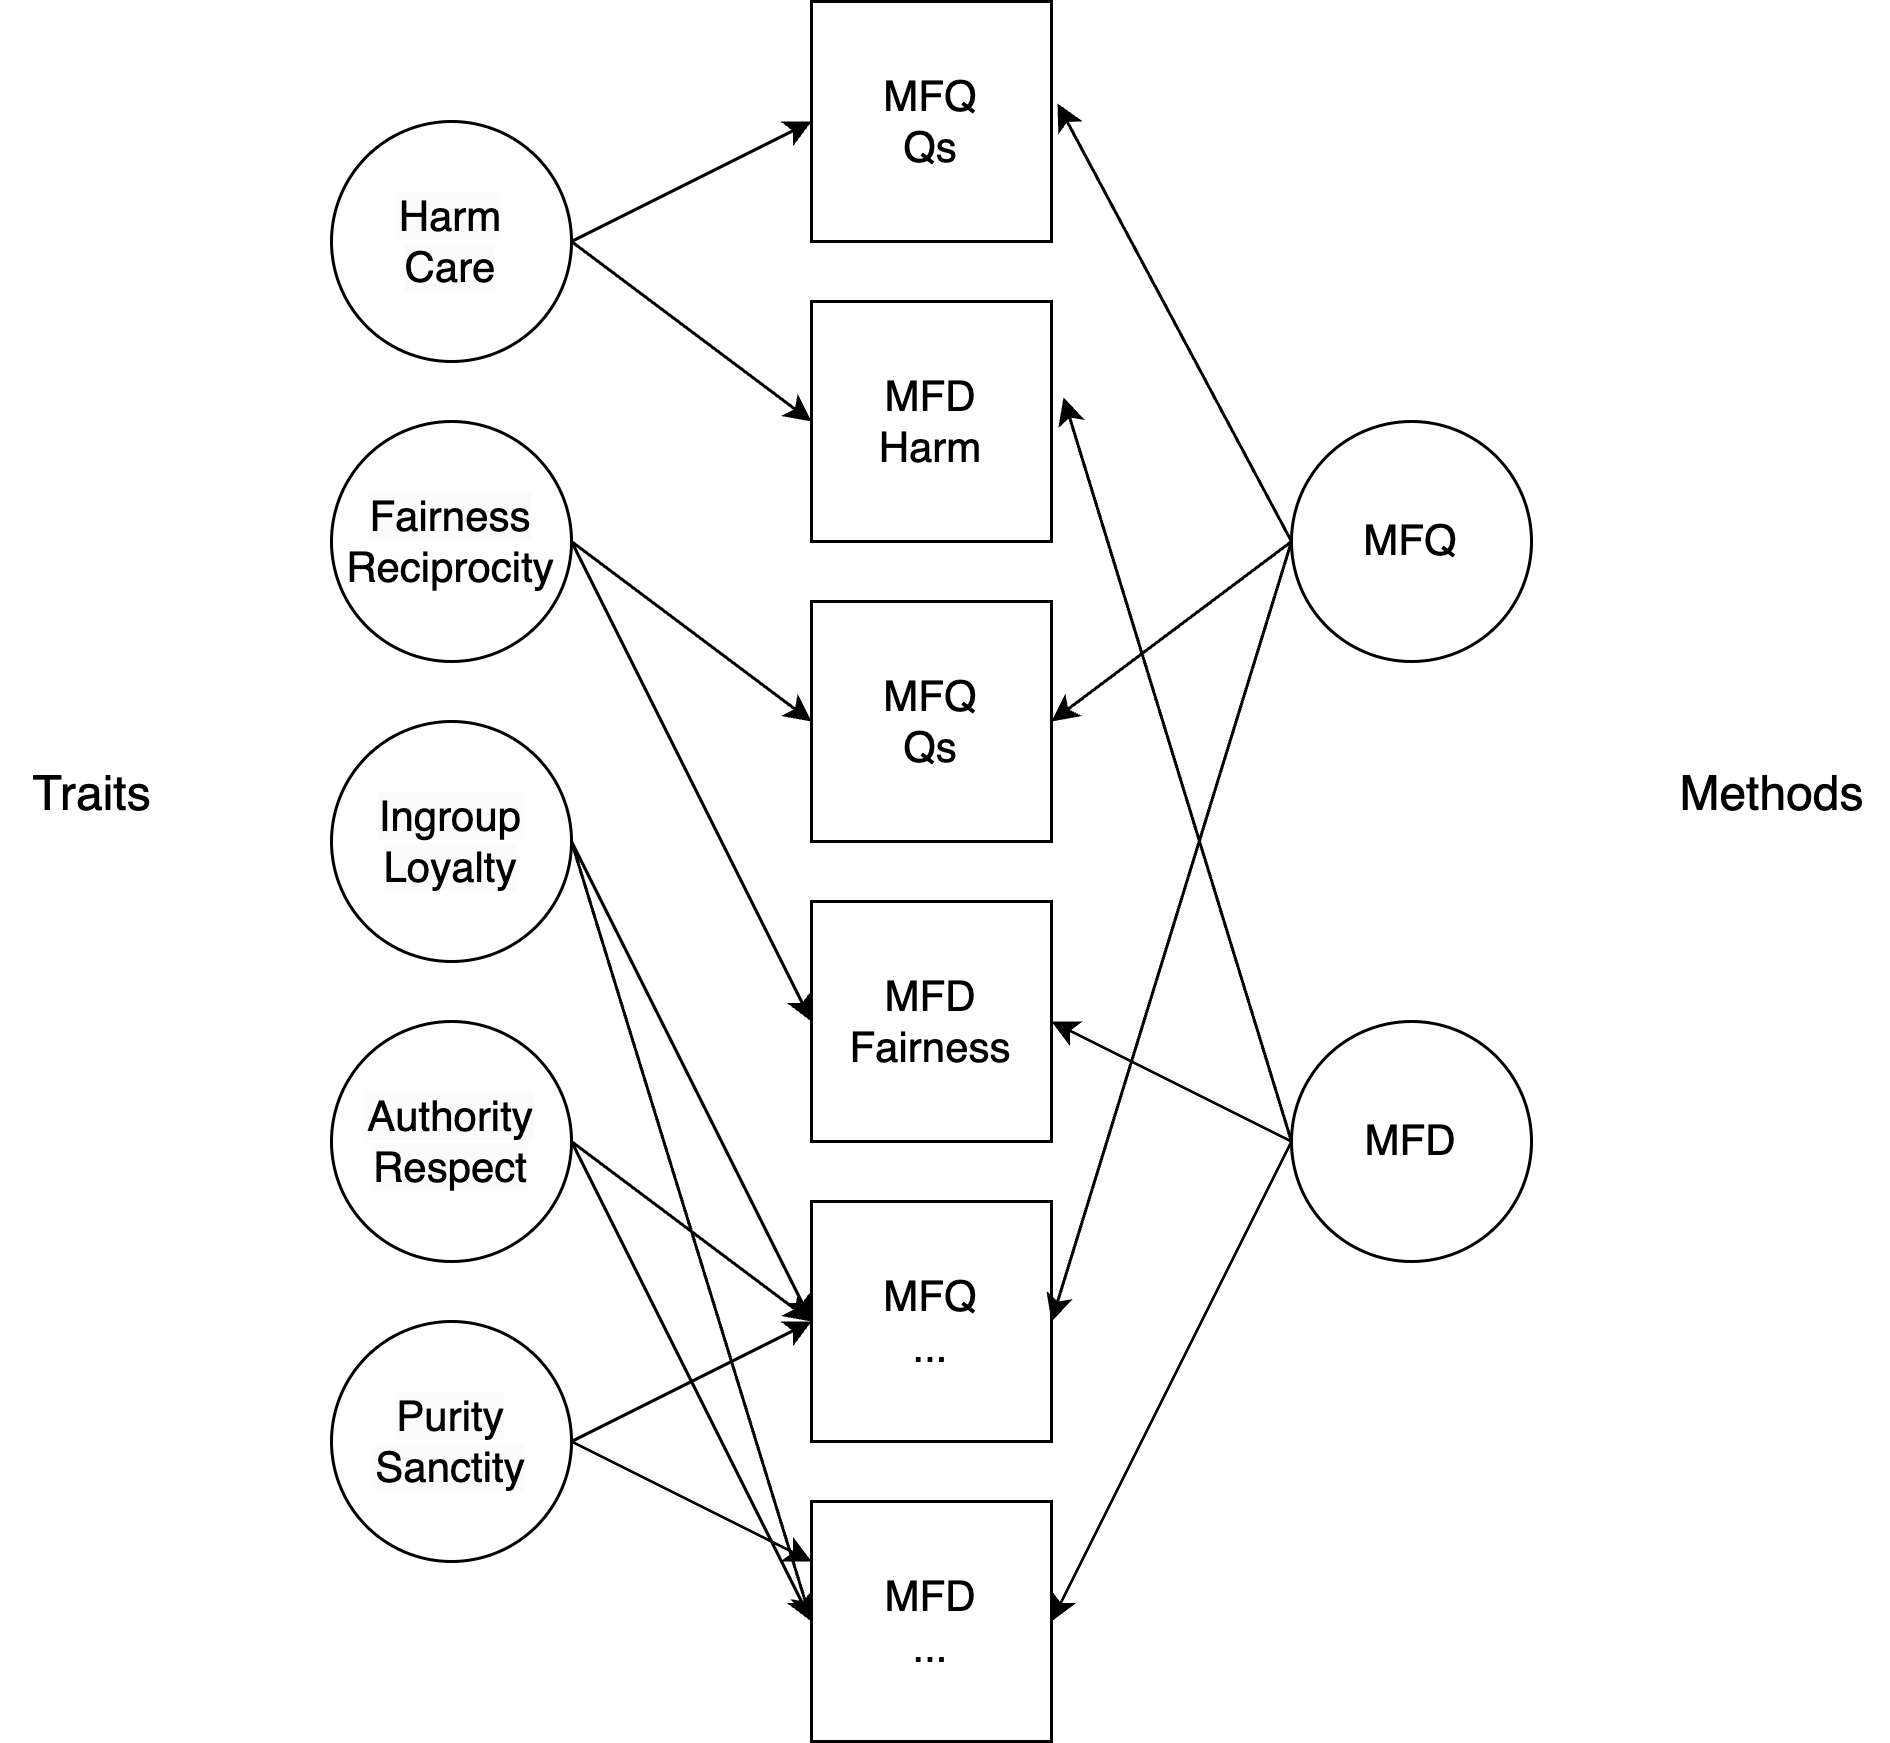
\includegraphics[width=6.3in]{mtmm_mfd} \caption{Representation of the multi-trait multi-method model for the MFD and MFQ. Not all measured variables (squares) are shown for ease of reading. The left hand side represents the traits or foundation areas of MFT, while the right hand side represents the two measurement tools for the MFT. }\label{fig:fig-mtmm}
\end{figure}

\subsubsection{Method}\label{method}

\paragraph{MFD Dictionaries}\label{mfd-dictionaries}

We created three versions of the MFD for separate MTMM analyses. The first dataset \emph{original MFD} was comprised of the original concepts from the MFD. We added all versions of the original words (i.e., abuse --\textgreater{} abusive, abuser, abused) to ensure all forms of the words were captured within the stemming procedure. These words where then stemmed using the same procedures as the data processing described for the overall study to match the data processing completed on the participant prompt responses in Study 1.2. The \emph{complete MFD} dataset included the original MFD concepts, all concepts listed from Study 1.1, and concepts from Study 1.2. The \emph{reduced MFD} dataset included all concepts from the original MFD, correlated concepts from Study 1.2, and concepts from Study 1.2 (only correlated concepts were selected in Study 1.2). The percent of concepts within each moral found area was calculated on the writing prompts from Study 1.2. The percent values were calculated on the processed data excluding all stop words. These values are represented as the MFD squares in Figure \ref{fig:fig-mtmm}.

\paragraph{MFQ Subscore}\label{mfq-subscore}

The MFQ individual questions for each participant were used from Study 1.2. These values are represented as the MFQ Qs squares in Figure \ref{fig:fig-mtmm}. The final number of participants included in this model was 387.

\paragraph{Models}\label{models}

For clarity, we programmed the following models:

\begin{enumerate}
\def\labelenumi{\arabic{enumi}.}
\tightlist
\item
  Model 1 \emph{Correlated Traits Correlated Methods}

  \begin{enumerate}
  \def\labelenumii{\alph{enumii}.}
  \tightlist
  \item
    \emph{Original} Original MFD Words
  \item
    \emph{Complete} Original MFD Words + Study 1.1 + Study 1.2 Words
  \item
    \emph{Reduced} Original MFD Words + Study 1.1 Reduced + Study 1.2 Words
  \item
    Determine if model suggests a feasible structure (fit indices
    adequate + loadings adequate)
  \item
    Pick the best model to continue (using model comparison)
  \end{enumerate}
\item
  Model 2 \emph{No Traits Correlated Methods}
\item
  Model 3 \emph{Perfectly Correlated Traits Correlated Methods}
\item
  Model 4 \emph{Correlated Traits Uncorrelated Methods}
\end{enumerate}

\subsubsection{Results}\label{results-2}

\begin{table}[ht]

\begin{center}
\begin{threeparttable}

\caption{\label{tab:tab-mtmm}Mean Percent Scores and MFQ Scores for Foundation Areas}

\footnotesize{

\begin{tabular}{llcc}
\toprule
Foundation Area & Dictionary/MFQ & M & SD\\
\midrule
Authority & MFQ & 11.52 & 3.06\\
Authority & Original & 0.37 & 0.62\\
Authority & Complete & 3.88 & 2.12\\
Authority & Reduced & 0.98 & 1.06\\
Fair & MFQ & 14.12 & 2.78\\
Fair & Original & 1.05 & 0.95\\
Fair & Complete & 4.94 & 2.37\\
Fair & Reduced & 3.16 & 1.85\\
Harm & MFQ & 13.85 & 2.79\\
Harm & Original & 1.13 & 1.21\\
Harm & Complete & 7.17 & 3.05\\
Harm & Reduced & 3.97 & 2.24\\
Ingroup & MFQ & 11.96 & 3.24\\
Ingroup & Original & 0.97 & 1.40\\
Ingroup & Complete & 5.12 & 2.63\\
Ingroup & Reduced & 1.69 & 1.67\\
Purity & MFQ & 11.69 & 3.61\\
Purity & Original & 0.73 & 0.82\\
Purity & Complete & 3.92 & 2.20\\
Purity & Reduced & 1.94 & 1.46\\
\bottomrule
\addlinespace
\end{tabular}

}

\begin{tablenotes}[para]
\normalsize{\textit{Note.} Mean percents for dictionaries, mean total subscores for the MFQ.}
\end{tablenotes}

\end{threeparttable}
\end{center}

\end{table}

Table \ref{tab:tab-mtmm} indicates the average percents found for each dictionary within each moral foundation area. The original MFD shows the lowest percentage of moral words for each foundation area, while the complete and reduced dataset show increases in the percent of text that would be considered moral words.

\paragraph{Model 1}\label{model-1}

Fit indices from the MTMM Model 1 step are shown in Table \ref{tab:mtmm-model1-table}. The complete parameter estimates from these models are saved online for full inspection due to their length. The fit indices from these models indicate that all models showed good fit. The original and complete MFD models showed equal fit (\(\Delta\) CFI \textless= .01), and both models were better than the reduced MFD model. We then inspected the loadings to determine the adequacy of the loadings for the MFQ and MFD. These results are shown in Table \ref{tab:mtmm-model1-table2}. All but one question for the MFQ load adequately (\textgreater.30; \emph{denied rights}) on each of their moral foundation areas. None of the MFD areas load onto their moral foundation area, as all loadings are close to zero (and non-significant, see online). The excellent model fit was likely due to the structure of the MFQ, as the MFD results do not show relation to their foundation area. We did not run further models, as the goal was to show that Model 1 was the best model with appropriate loadings for foundations.

\begin{table}[ht]

\begin{center}
\begin{threeparttable}

\caption{\label{tab:mtmm-model1-table}MTMM Fit Indices for Model 1 MTMM}

\footnotesize{

\begin{tabular}{llccllcc}
\toprule
Model & Chi-Sq & df & RMSEA & SRMR & CFI & TLI & AIC\\
\midrule
Original & 204.40 & 71.00 & 0.03 & 0.04 & 0.98 & 0.97 & 21,575.55\\
Complete & 239.09 & 71.00 & 0.04 & 0.04 & 0.97 & 0.96 & 24,868.17\\
Reduced & 283.10 & 71.00 & 0.05 & 0.05 & 0.95 & 0.94 & 23,380.58\\
\bottomrule
\end{tabular}

}

\end{threeparttable}
\end{center}

\end{table}

\begin{table}[ht]

\begin{center}
\begin{threeparttable}

\caption{\label{tab:mtmm-model1-table2}MTMM Parameter Estimates for Model 1 Loadings}

\footnotesize{

\begin{tabular}{llccl}
\toprule
Latent Variable & Measured Variable & Original & All & Reduced\\
\midrule
Harm & Emotional Suffering & 0.61 & 0.61 & 0.61\\
Harm & Cared for Weak & 0.70 & 0.69 & 0.69\\
Harm & Cruel & 0.38 & 0.37 & 0.36\\
Harm & MFD & -0.05 & -0.03 & -0.05\\
Fair & Treated Differently & 0.76 & 0.76 & 0.77\\
Fair & Acted Unfairly & 0.52 & 0.50 & 0.50\\
Fair & Denied Rights & 0.23 & 0.22 & 0.22\\
Fair & MFD & -0.01 & 0.10 & 0.05\\
Ingroup & Love for Country & 0.63 & 0.63 & 0.63\\
Ingroup & Betray Group & 0.73 & 0.72 & 0.73\\
Ingroup & Lack of Loyalty & 0.82 & 0.81 & 0.81\\
Ingroup & MFD & -0.10 & 0.03 & 0.05\\
Authority & Lack of Respect & 0.81 & 0.80 & 0.81\\
Authority & Conformed to Tradition & 0.72 & 0.72 & 0.72\\
Authority & Chaos or Disorder & 0.42 & 0.41 & 0.41\\
Authority & MFD & 0.06 & 0.00 & -0.04\\
Purity & Purity and Decency & 0.71 & 0.71 & 0.71\\
Purity & Disgusting & 0.67 & 0.67 & 0.67\\
Purity & Acted God & 0.64 & 0.64 & 0.64\\
Purity & MFD & 0.06 & -0.05 & -0.11\\
\bottomrule
\addlinespace
\end{tabular}

}

\begin{tablenotes}[para]
\normalsize{\textit{Note.} Estimates are completely standardized loadings from the model.}
\end{tablenotes}

\end{threeparttable}
\end{center}

\end{table}

\subsection{Discussion}\label{discussion}

Study 1 was designed to investigate if the original MFD could be improved with additional concepts. As shown in Table \ref{tab:tab-mtmm}, the original MFD is often heavily skewed toward zero with very low percentages of moral words used in text. These results were found even when writing about concepts that should theoretically active moral values. The suggested improvements did increase percentages of included words; however, the results from the MTMM indicate that the MFD does not appear to relate to the MFQ moral foundations. In a separate set of studies, we examined if the original MFD proposed results for liberal and conservative values could be found within new sources (Sagi \& Dehghani, 2014). Further, we examined if the MFD could be improved with markers of valence (i.e., positive, negative), rather than just inclusion of more words.

\section{Study 2}\label{study-2}

\subsection{Method}\label{method-1}

We hypothesized the news sources generally perceived as liberal leaning
(\emph{NPR} and \emph{The New York Times}) would contain MFD words and valences
indicating endorsements of the individualizing moral foundations
(harm and fairness), and thus, higher foundation scores in this area than conservative sources (Sagi \& Dehghani, 2014). Additionally, we hypothesized that the two sources generally perceived to be conservative leaning (\emph{Fox News} and \emph{Breitbart}) would feature MFD words and valences with higher scores in the authority and purity areas. Given the previously mixed results of ingroup, we do not make a directional prediction (Frimer, 2020).

\subsubsection{Sources}\label{sources}

Political articles were collected from the websites of four notable U.S.
news sources, a process known as web scraping. The sources were \emph{NYT},
\emph{NPR}, \emph{Fox News}, and \emph{Breitbart}. They were selected for their
widespread recognition and the fact political partisans have strong
preferences for some sources over others. We determined the political
lean of each source by referencing Mitchell, Matsa, Gottfried, and Kiley (2014)'s article demonstrating
the self-reported ideological consistency represented by the consumers
of several news sources. In general, the \emph{NYT} and \emph{NPR} are preferred
by consumers reporting a liberal bias or lean. In contrast, \emph{Fox News}
and \emph{Breitbart} are believed to have a conservative bias or lean.
Mitchell et al. (2014)'s article presented political ideology as a scale ranging
from ``consistently liberal'' to ``consistently conservative.'' In between
these extremes lie more moderate positions, including ``mostly liberal,''
``mixed,'' and ``mostly conservative.'' Owing to the lower number of sources
analyzed herein, we elected to categorize the sources as either
``liberal'' and ``conservative'' in order to form a basis for comparison. At
the time of our data collection, these sources were also selected
because they were open (i.e., no subscription required to access
articles), and their websites were designed in a way that made
webscraping possible.

Political articles in particular were identified and subsequently
scraped by including the specific URL directing to each source's
political content in the \emph{R} script. For example, rather than scrape
from nytimes.com, which would return undesired results (non-political
features, reviews, etc.), we instead included
nytimes.com/section/politics so that more or less exclusively political
content was obtained. All code for this manuscript can be found at
\url{https://osf.io/5kpj7/}, and the scripts are provided inline with this
manuscript written with the \emph{papaja} library (Aust \& Barth, 2017).

Identification of the sources' political URLs presented a problem for
two of the sources owing to complications with how their particular
sites were structured. While in the multi-week process of scraping
articles, we noticed word counts for \emph{NPR} and \emph{Fox News} were not
growing at a similar pace as those from the \emph{NYT} and \emph{Breitbart}. Upon
investigation, we found another, more robust URL for political content
from NPR: their politics content archive. The page structure on NPR's
website was such that only a limited selection of articles is displayed
to the user at a given time. Scraping both the archive and the normal
politics page ensured we were obtaining most (if not all) new articles
as they were published. We later ran a process in order to exclude any
duplicate articles. \emph{Fox News} presented a similar issue. We discovered
\emph{Fox News} utilized six URLs in addition to the regular politics page.
These URLs led to pages containing content pertaining the U.S. Executive
Branch, Senate, House of Representatives, Judicial Branch, foreign
policy, and elections. Once again, duplicates were subsequently
eliminated from any analyses.

\subsubsection{Materials}\label{materials}

Using the \emph{rvest} library in the statistical package \emph{R}, we pulled body
text for individual articles from each of the aforementioned sources
(identified using CSS language) and compiled them into a dataset
(Wickham, 2016). Using this dataset, we identified word count and average
word count per source. This process was completed once daily starting in
February 2018 until March 2018. Starting in mid-March 2018, the process
was completed twice daily - once in the morning and again in the
evening. Data collection was terminated once 250,000 words per source
was collected in April 2018.

\subsubsection{Data Analysis}\label{data-analysis}

Once data collection ended, the text sources and Warriner, Kuperman, and Brysbaert (2013) dataset were processed as described in Study 1. The words making up each of the five foundations in the MFD were matched to their respective valence value. The Warriner et al. (2013) data includes nearly 14,000 English lemmas that have
been rated for their valence, arousal, and dominance (mirroring Bradley \& Lang, 1999). Word emotion ratings have been used to estimate the
sentiment of a text - a very popular task within classification
research - by generally averaging the valence scores of the the words
matched between the text and the available norms (Leveau, Jhean-Larose, Denhière, \& Nguyen, 2012). Other
suggestions include the simple summation of word's positive or negative
valence from a text or respective weighting based on word frequency
(Hutto, 2021; Loria, 2020). In each of these cases, an overall polarity is
desired, which is the case here, creating an overall score for each of
the five MFD domains. Sentiment coding packages often score items from
-1 to 1 or other values around zero wherein negative scores represent
negative sentiment, while positive scores represent positive sentiment.
The Warriner et al. (2013) dataset ranges from 1 (\emph{unhappy}) to 9 (\emph{happy}).
Thus, to ensure that we anchored their valences around zero, we
\emph{z}-scored the dataset so that negative scores represented values below
the average sentiment and positive scores represented values above the
average sentiment.

Given the results from Study 1.3, we used the original MFD to calculate
the number of words included for each moral foundation area. We could
also suggest using the larger complete dataset, given that the CFI indicated
similar models. The total number of times each of those words
was used in an article was calculated. This information was merged with
the valence values from the Warriner et al. (2013) dataset. A weighted score was
calculated by multiplying the frequency of occurrence within a document
times the \emph{z}-scored valence values and divided by the word count for
that article. The final score was multiplied by 100 to represented a
weighted percentage. Finally, the weighted scores were summed within in
each article to get a total weighted percentage of the use of moral area
specific words by article. Valences were \emph{z}-scored in order to
eliminate any ambiguity regarding the direction of the valence. Positive
values indicate positive valence, and negative values indicate negative
valence. Words were categorized in accordance to their MFD affiliation,
creating a weighted sum for each moral foundation. See Table
\ref{tab:example-weight} for an example.

\begin{table}[ht]

\begin{center}
\begin{threeparttable}

\caption{\label{tab:example-weight}Example of Weighted Coding for Harm Words}

\footnotesize{

\begin{tabular}{llcccc}
\toprule
Source & Concept & Frequency & Total Words & Valence & Weighted Score\\
\midrule
Breitbart & defend & 4.00 & 341 & 0.97 & 1.14\\
NPR & protect & 11.00 & 1550 & 1.39 & 0.98\\
NPR & fight & 7.00 & 10740 & -1.20 & -0.08\\
NPR & violenc & 11.00 & 1419 & -1.85 & -1.43\\
Breitbart & safe & 4.00 & 1108 & 2.07 & 0.75\\
Breitbart & sympathet & 1.00 & 1632 & 1.26 & 0.08\\
Breitbart & benefit & 6.00 & 1774 & 1.42 & 0.48\\
NY Times & care & 19.00 & 4422 & 2.02 & 0.87\\
NY Times & harm & 4.00 & 1100 & -2.47 & -0.90\\
Breitbart & damag & 4.00 & 1624 & -1.63 & -0.40\\
Breitbart & preserv & 2.00 & 254 & 1.27 & 1.00\\
NY Times & destroy & 5.00 & 1494 & -1.88 & -0.63\\
NY Times & spurn & 1.00 & 1508 & NA & NA\\
Breitbart & cruel & 2.00 & 574 & -1.83 & -0.64\\
Breitbart & violent & 6.00 & 1211 & -2.20 & -1.09\\
\bottomrule
\addlinespace
\end{tabular}

}

\begin{tablenotes}[para]
\normalsize{\textit{Note.} Concepts were stemmed to match datasets. The frequency was divided by the total numbers and then multiply by valence and 100 to create percent weighted scores.}
\end{tablenotes}

\end{threeparttable}
\end{center}

\end{table}

\subsection{Results}\label{results-3}

Descriptive and test statistics, \emph{p}-values and effect sizes (Cohen's
\(d_s\)) can be found in Table \ref{tab:exp1-table}. To interpret the
weighted scores, one can examine the mean and standard deviations for
each. A zero score for the mean, with a non-zero standard deviation,
would indicate a perfect balance of positive and negative words in each
category, likely representing a neutral sentiment when all words are
considered. Negative percentages would indicate more representation of
the negative words in the MFD area, while positive percentages indicate
an endorsement of the positive words in a MFD. Therefore, we suggest
using the sign of the mean score to determine the directionality of the
endorsement for the MFD (positive, neutral, negative), and the standard
deviation to ensure that a zero score is not zero endorsement (i.e., a
SD of zero indicates no words were used).

To analyze if news sources adhered to differences in word use based on
their target audience, we utilized a multilevel model (MLM) to analyze
the data. MLM is a regression technique that allows one to control for
the repeated measurement and nested structured of the data, which
creates correlated error (Gelman, 2006). Using the \emph{nlme} library in \emph{R}
(Pinheiro, Bates, Debroy, Sarkar, \& Team, 2017), each foundation's weighted percentage was predicated
here by the political lean of the news source, using the individual news
sources as a random intercept to control for the structure of the data.
Therefore, the models were calculated by: \texttt{Weighted\ Score\ (or\ Original\ Percent\ Score)\ \textasciitilde{}\ Political\ Lean\ +\ (\textasciitilde{}1\textbar{}Source)}. Both the valence weighted scores and original MFD scores were used as dependent variables to compare results across different scorings of the MFD. The multilevel model did not indicate the presence of any significant effects for political lean for any of the five moral
foundations. The effect sizes (\(d_s\)) appear to show a similar pattern of results, but given that most are close to zero, it is difficult to know if these two scoring systems showed similar results or these results were simply null effects. The original scoring shows a small effect size for purity (considering that previous effect sizes reported were .50+, we considered .20 small) in the expected direction.

\begin{table}[ht]

\begin{center}
\begin{threeparttable}

\caption{\label{tab:exp1-table}News Source Results - Multilevel Model}

\footnotesize{

\begin{tabular}{lccccccclc}
\toprule
Model & Foundation & $M_C$ & $SD_C$ & $M_L$ & $SD_L$ & $t$ & $p$ & $d_s$ & ICC\\
\midrule
Valence & Harm & -0.49 & 1.26 & -0.44 & 1.26 & 0.50 & .668 & -0.04 & .001\\
Valence & Fairness & 0.47 & 0.64 & 0.44 & 0.64 & -1.23 & .344 & 0.05 & < .001\\
Valence & Ingroup & 0.39 & 0.49 & 0.38 & 0.49 & -0.58 & .620 & 0.02 & < .001\\
Valence & Authority & 0.09 & 0.49 & 0.07 & 0.49 & -1.25 & .338 & 0.05 & < .001\\
Valence & Purity & 0.19 & 0.53 & 0.13 & 0.53 & -2.77 & .109 & 0.10 & .001\\
Original & Harm & 0.55 & 0.60 & 0.50 & 0.60 & -1.84 & .207 & 0.07 & < .001\\
Original & Fairness & 0.46 & 0.49 & 0.41 & 0.49 & -2.57 & .124 & 0.10 & .003\\
Original & Ingroup & 0.63 & 0.64 & 0.68 & 0.64 & 1.83 & .208 & -0.07 & .002\\
Original & Authority & 0.67 & 0.70 & 0.60 & 0.70 & -2.28 & .150 & 0.09 & < .001\\
Original & Purity & 0.17 & 0.32 & 0.11 & 0.32 & -3.78 & .064 & 0.20 & .009\\
\bottomrule
\addlinespace
\end{tabular}

}

\begin{tablenotes}[para]
\normalsize{\textit{Note.} For mean and standard deviation values, 'C' and 'L' refer to 'conservative' and 'liberal,' respectively}
\end{tablenotes}

\end{threeparttable}
\end{center}

\end{table}

\subsection{Discussion}\label{discussion-1}

The results obtained in Study 2 fail to support most of the predicted differences
predicted by MFT. First, differences between liberal and conservative
news sources failed to reach statistical or practical (effect size)
significance for nearly all foundations. One effect was in the predicted direction, with higher endorsement for purity words in the conservative sources. One possible limitation of the current data is the generalness
of the corpus. The selection of the broad and amorphous topic of
``political news'' may have led to the scraping of large numbers of
articles with little to no moral-centric content. To address this
limitation, two changes that were subsequently employed in Study 3.
First, we elected to include more news sources for web scraping and
analysis in addition to the four used in Study 2. Second, we chose to
focus data collection efforts on two heavily moralized events in the
Trump administration: (1) the nomination and confirmation of Justice
Brett Kavanaugh to the U.S. Supreme Court and the U.S. government
shutdown in December 2018 through January 2019 over disagreements about
funding a U.S.-Mexico border wall. Hence, Study 3 was an improved test of
the MFT and the MFD in the context of partisan news.

\section{Study 3}\label{study-3}

\subsection{Method}\label{method-2}

We tested the same hypotheses as described in Study 2 by analyzing the content scraped from news sources' web pages spanning the two weeks before (September 13, 2018) and two weeks after (October 11, 2018) Kavanaugh's confirmation hearing, owing to its prominence in the news. Likewise, we analyzed content
spanning two weeks before the start of the government shutdown (December
8, 2018) to two weeks following the end of the shutdown (February 8,
2019).

\subsubsection{Sources}\label{sources-1}

Articles pertaining to the Brett Kavanaugh Supreme Court confirmation
hearing and the 2018-2019 U.S. Government shutdown were scraped from the
websites of 10 U.S. news sources. As in Study 2, these sources were
selected owing to their favorability among political partisans according
to Mitchell et al. (2014). The sources favored by the highest proportion of
consistent liberals were the \emph{NYT}, \emph{NPR}, \emph{Slate}, \emph{Huffington Post},
and \emph{Politico} (Mitchell et al., 2014). The sources favored by the highest
proportion of consistent conservatives included \emph{Fox News}, \emph{Breitbart},
\emph{The Rush Limbaugh Show}, \emph{The Blaze}, and \emph{Sean Hannity}. These sources
were primarily selected due to their political lean but also due to our
ability to webscrape their contents without a subscription based
service.

\subsubsection{Materials}\label{materials-1}

Using the \emph{rvest} and \emph{RSelenium} libraries, we pulled body text for
individual articles from each of the aforementioned 10 news sources and
compiled them together (Harrison \& Kim, 2020; Wickham, 2016). Kavanaugh's widely-publicized and viewed nomination hearing was on September 27, 2018. We set the start date at September 13 (two weeks before the hearing) and the end date at October 11 (two weeks after the hearing) so that we
could capture a large amount of data (roughly one month) during which
Kavanaugh's nomination was at its peak saturation in news coverage. The same process was followed for scraping articles related to the
partial U.S. Government shutdown of 2018-2019. The articles scraped were
published between December 8, 2018 and February 8, 2019 inclusive. Once
again, we elected to scrape articles published two weeks before and
after the event in question in order to capitalize on the shutdown's
saturation in American news media.

\subsubsection{Data analysis}\label{data-analysis-1}

The data analysis used the same procedure as Study 1 for preparing the text, and the same weighting procedure described in Study 2 for creating valence scores.

\subsection{Results}\label{results-4}

The same multilevel models were used to calculate the differences in news sources political lean across foundation areas using either valence weighted scoring or original MFD scoring (see Study 2 for model code).

The pattern of results is nearly identical when examining \(d_s\) scores for standardization, as the scorings are set on different scales (see Table \ref{tab:exp2-tablekav}). A few significant results were found: 1) higher fairness scores for conservatives \(d_s\) \textasciitilde{} .40s (both), 2) higher purity scores for conservatives \(d_s\) \textasciitilde{} .47s (original score significant, weighted scores non-significant, but effect sizes were nearly identical). In general, the variance is a bit larger for the weighted scores, which may lead to the differences in traditional significance interpretations, and we advise examining effect sizes for interpretation. The rest of the effects were nearly zero.

\begin{table}[ht]

\begin{center}
\begin{threeparttable}

\caption{\label{tab:exp2-tablekav}Kavanaugh Results - Multilevel Model}

\footnotesize{

\begin{tabular}{llcccccccl}
\toprule
Model & Foundation & $M_C$ & $SD_C$ & $M_L$ & $SD_L$ & $t$ & $p$ & $d_s$ & ICC\\
\midrule
Valence & Harm & -0.35 & 0.69 & -0.32 & 0.69 & 0.58 & .575 & -0.04 & .013\\
Valence & Fairness & 0.91 & 0.74 & 0.60 & 0.74 & -2.68 & .028 & 0.42 & .095\\
Valence & Ingroup & 0.24 & 0.31 & 0.25 & 0.31 & 0.31 & .764 & -0.03 & .004\\
Valence & Authority & 0.04 & 0.32 & 0.06 & 0.32 & 1.08 & .313 & -0.06 & .003\\
Valence & Purity & 0.36 & 0.51 & 0.16 & 0.51 & -1.75 & .118 & 0.47 & .133\\
Original & Harm & 0.33 & 0.36 & 0.35 & 0.36 & 0.60 & .567 & -0.04 & .010\\
Original & Fairness & 0.77 & 0.57 & 0.54 & 0.57 & -2.84 & .022 & 0.40 & .142\\
Original & Ingroup & 0.34 & 0.37 & 0.37 & 0.37 & 0.35 & .733 & -0.06 & .010\\
Original & Authority & 0.43 & 0.49 & 0.46 & 0.49 & 1.20 & .266 & -0.04 & .004\\
Original & Purity & 0.28 & 0.31 & 0.15 & 0.31 & -2.44 & .040 & 0.49 & .126\\
\bottomrule
\addlinespace
\end{tabular}

}

\begin{tablenotes}[para]
\normalsize{\textit{Note.} For mean and standard deviation values, 'C' and 'L' refer to 'conservative' and 'liberal,' respectively.}
\end{tablenotes}

\end{threeparttable}
\end{center}

\end{table}

For news articles about the partial U.S. Federal Government Shutdown of
2018-2019, only one significant effect was found (see Table \ref{tab:exp2-tablegs}). The original scoring for fairness indicated that conservatives endorsed more fairness related words \(d_s\) = 0.75. The valence weighted scoring showed the same effect size \(d_s\) = 0.74, but was non-significant in traditional null hypothesis testing interpretations. Both effects would be considered large and in line with previous findings, \emph{except} in the opposition direction of predicted results. The same large effects can be found for the purity foundation \(d_s\) = 0.85 (both), in the expected direction that conservative sources endorsed more purity words than liberal sources.

\begin{table}[ht]

\begin{center}
\begin{threeparttable}

\caption{\label{tab:exp2-tablegs}Government Shutdown Results - Multilevel Model}

\footnotesize{

\begin{tabular}{llcccccccl}
\toprule
Model & Foundation & $M_C$ & $SD_C$ & $M_L$ & $SD_L$ & $t$ & $p$ & $d_s$ & ICC\\
\midrule
Valence & Harm & -0.13 & 0.70 & -0.15 & 0.70 & -0.55 & .594 & 0.03 & .008\\
Valence & Fairness & 0.79 & 0.57 & 0.40 & 0.57 & -1.57 & .154 & 0.74 & .139\\
Valence & Ingroup & 0.35 & 0.39 & 0.37 & 0.39 & 0.53 & .611 & -0.05 & .012\\
Valence & Authority & 0.03 & 0.33 & 0.03 & 0.33 & 0.67 & .524 & -0.01 & .004\\
Valence & Purity & 0.48 & 0.49 & 0.08 & 0.49 & -1.38 & .206 & 0.85 & .155\\
Original & Harm & 0.34 & 0.38 & 0.36 & 0.38 & 1.24 & .251 & -0.04 & < .001\\
Original & Fairness & 0.68 & 0.44 & 0.38 & 0.44 & -2.35 & .047 & 0.75 & .148\\
Original & Ingroup & 0.51 & 0.50 & 0.54 & 0.50 & 0.23 & .825 & -0.06 & .015\\
Original & Authority & 0.42 & 0.44 & 0.43 & 0.44 & 0.58 & .578 & -0.02 & .002\\
Original & Purity & 0.34 & 0.30 & 0.13 & 0.30 & -1.38 & .206 & 0.85 & .155\\
\bottomrule
\addlinespace
\end{tabular}

}

\begin{tablenotes}[para]
\normalsize{\textit{Note.} For mean and standard deviation values, 'C' and 'L' refer to 'conservative' and 'liberal,' respectively.}
\end{tablenotes}

\end{threeparttable}
\end{center}

\end{table}

\subsection{Discussion}\label{discussion-2}

The results obtained in Study 3 portrayed that focused news sources may provide a bit more evidence for the MFD to assess MFT's predictions, at least for purity. This result showed a large effect, and depending on the scoring, sometimes the traditional significance matching results from Graham et al. (2009). The results for fairness were in the opposite direction of expectations, given the MFT and previous studies, where we found that conservatives endorsed more fairness words than liberal sources. Study 2 and 3's results indicated that the effect sizes will likely be similar for either the traditional percent or weighted scoring, as they are nearly identical in each study. We suggest using the simpler percent scoring, which can be calculated with both programming software \emph{R} and point and click software LIWC (Pennebaker et al., 2007).

\section{Conclusions}\label{conclusions}

Within the theoretical framework of MFT (Haidt \& Graham, 2007), we attempted to improve the MFD (Graham et al., 2009) and demonstrate its relation with other reliable measurements of moral foundations, the MFQ. In Study 1, we examined potential new concepts to add to the MFD by collecting word associations and moral related texts from participants. Several dictionary improvements were suggested, but the results of a multi-trait multi-method analysis indicate that the MFD does not relate to the moral foundations found in the MFD. Therefore, we did not find support for the use of the MFD in relation to the MFQ using a convergent and divergent validity technique.

In Study 2 and 3, we attempted to
devise a method leveraging the MFD and valence weighting in order to replicate previous effects on political bias stemming from content published by several prominent American news sources. In Study 2, we only discovered a small effect for purity, while all other results obtained were not
significant in any statistical or practical sense. This result was replicated in Study 3 with a larger effect size, along with differences found in fairness, albeit in the opposite direction than predicted. Building on Frimer (2020) and other critiques of MFT and the MFD, we show that MFD may not yet be a useful tool for measuring moral language while also calling into question the validity of MFT in terms of theorized partisan differences.

The results from different proposed scoring methods remained consistent with the original percent scoring method. This scoring may provide insight into the sentiment of the texts. For example, the harm foundation is considered a continuum ranging from harm to care. The results from Study 2 and 3 indicate that the MFD likely measures more harm than care across the continuum in our sources. In general, given that the weighted valence scoring requires more sophisticated programming skills to implement, we suggest using the original scoring of the MFD with all results taken together.

Political lean and other important political/moral constructs
may be communicated through methods other than through the use of
particular words. As mentioned before, MFD is a measure developed from
MFT (Graham et al., 2009). Based upon the results obtained, it might be
necessary to investigate alternative instruments that could better
elucidate the differences of interest. Going beyond specific
instruments, other theoretical perspectives may be more equipped to
explain political differences in discourse. Likewise, an atheoretical
approach in which large quantities of data are collected from which
theories are formulated may be best suited to this area of research.

In critiquing the MFT, Schein and Gray (2015) proposed an alternative theory explaining
moral choices and potential partisan differences: Dyadic Theory of
Morality. Across many studies, researchers find that supposed
differences in moral foundation can be more easily explained by a
harm-focused morality where someone/thing is harmed by someone/thing
else (Gray, Schein, \& Ward, 2014; Schein \& Gray, 2015). Rather than liberals and conservatives
having difference conceptions of morality, dyadic morality argues that
they simply identify harm differently. For example, in the case of
abortion, liberals tend to identify the primary harm to the mother
leading to a pro-choice position whereas conservative tend to identify
the primary harm to the fetus leading to a pro-life position. While as
of yet, no linguistic measurement of dyadic morality exists; such an
approach may be able to better identify the systematic differences
between liberals and conservatives.

Turning to atheoretical approaches, future studies aiming to uncover
political lean in discourse may benefit from a bottom-up, data-driven
approach. Researchers might derive substantive insights into political
lean through gathering data after which they may formulate theories that
explain systematic observations obtained from that data. The
availability of text corpora along with methods for extracting large
amounts of text from the internet (as was demonstrated in the current
study) potentially make this a feasible option. Likewise, there are
several approaches to analyzing such data, including linear models (like
multilevel models) and network-style models such as latent semantic
analysis (Landauer, 1998). Owing to the wealth of representative data as
well as the sophistication of current analytic tools, there is high
potential for the explanatory power of new theories involving political
discourse.

Never before has political discourse represented such fertile ground for
psychological research. The plethora of options for news sources has
created not only an abundance of choice but also vast quantities of text
data. Along with this recent increase in the amount of text information,
there is now an obligation on the part of researchers to devise proper
methods for analyzing that text. Solid methodologies must be constructed
and periodically improved to keep pace with evolving technologies.
Likewise, a strong theoretical foundation is paramount to making sense
of the current and future media ecosystem. Therefore, it is incumbent
upon social scientists to continue investigating the information
consumed by millions of Americans every day so that insights into the
nature and consequences of political discourse can be more completely
understood.

\newpage

\section{References}\label{references}

\phantomsection\label{refs}
\begin{CSLReferences}{1}{0}
\bibitem[\citeproctext]{ref-Aust2017}
Aust, F., \& Barth, M. (2017). \emph{{papaja: Create APA manuscripts with R Markdown.}} Retrieved from \url{https://github.com/crsh/papaja}

\bibitem[\citeproctext]{ref-bentler1990}
Bentler, P. M. (1990). Comparative fit indexes in structural models. \emph{Psychological Bulletin}, \emph{107}(2), 238--246. \url{https://doi.org/10.1037/0033-2909.107.2.238}

\bibitem[\citeproctext]{ref-bentler1980}
Bentler, P. M., \& Bonett, D. G. (1980). Significance tests and goodness of fit in the analysis of covariance structures. \emph{Psychological Bulletin}, \emph{88}(3), 588--606. \url{https://doi.org/10.1037/0033-2909.88.3.588}

\bibitem[\citeproctext]{ref-bradley1999}
Bradley, M. M., \& Lang, P. J. (1999). \emph{Affective Norms for English Words (ANEW): Instruction Manual and Affective Ratings}. The Center for Research in Psychophysiology.

\bibitem[\citeproctext]{ref-buuren2011}
Buuren, S. V., \& Groothuis-Oudshoorn, K. (2011). {\textbf{mice}} : Multivariate Imputation by Chained Equations in {\emph{R}}. \emph{Journal of Statistical Software}, \emph{45}(3). \url{https://doi.org/10.18637/jss.v045.i03}

\bibitem[\citeproctext]{ref-byrne2001}
Byrne, B. M. (2001). Structural Equation Modeling With AMOS, EQS, and LISREL: Comparative Approaches to Testing for the Factorial Validity of a Measuring Instrument. \emph{International Journal of Testing}, \emph{1}(1), 55--86. \url{https://doi.org/10.1207/S15327574IJT0101_4}

\bibitem[\citeproctext]{ref-Clifford2013}
Clifford, S., \& Jerit, J. (2013). How words do the work of politics: Moral foundations theory and the debate over stem cell research. \emph{The Journal of Politics}, \emph{75}(3), 659--671. \url{https://doi.org/10.1017/S0022381613000492}

\bibitem[\citeproctext]{ref-dedeyne2019}
De Deyne, S., Navarro, D. J., Perfors, A., Brysbaert, M., \& Storms, G. (2019). The {``}Small World of Words{''} English word association norms for over 12,000 cue words. \emph{Behavior Research Methods}, \emph{51}(3), 987--1006. \url{https://doi.org/10.3758/s13428-018-1115-7}

\bibitem[\citeproctext]{ref-Federico2013}
Federico, C. M., Weber, C. R., Ergun, D., \& Hunt, C. (2013). {Mapping the Connections between Politics and Morality: The Multiple Sociopolitical Orientations Involved in Moral Intuition}. \emph{Political Psychology}, \emph{34}(4), 589--610. \url{https://doi.org/10.1111/pops.12006}

\bibitem[\citeproctext]{ref-feinerer2008}
Feinerer, I., Hornik, K., \& Meyer, D. (2008). Text Mining Infrastructure in {\emph{R}}. \emph{Journal of Statistical Software}, \emph{25}(5). \url{https://doi.org/10.18637/jss.v025.i05}

\bibitem[\citeproctext]{ref-Frimer2020}
Frimer, J. A. (2020). Do liberals and conservatives use different moral languages? Two replications and six extensions of {G}raham, {H}aidt, and {N}osek's (2009) moral text analysis. \emph{Journal of Research in Personality}, \emph{84}, 103906. \url{https://doi.org/10.1016/j.jrp.2019.103906}

\bibitem[\citeproctext]{ref-Frimer2015}
Frimer, J. A., Tell, C. E., \& Haidt, J. (2015). Liberals condemn sacrilege too: The harmless desecration of {C}erro {T}orre. \emph{Social Psychological and Personality Science}, \emph{6}(8), 878--886. \url{https://doi.org/10.1177/1948550615597974}

\bibitem[\citeproctext]{ref-Garten2016}
Garten, J., Boghrati, R., Hoover, J., Johnson, K. M., \& Dehghani, M. (2016). Morality between the lines: Detecting moral sentiment in text. \emph{{Proceedings of IJCAI 2016 workshop on Computational Modeling of Attitudes}}.

\bibitem[\citeproctext]{ref-Gelman2006}
Gelman, A. (2006). {Multilevel (hierarchical) modeling: What it can and cannot do}. \emph{Technometrics}, \emph{48}(3), 432--435. \url{https://doi.org/10.1198/004017005000000661}

\bibitem[\citeproctext]{ref-Graham2009}
Graham, J., Haidt, J., \& Nosek, B. A. (2009). {Liberals and conservatives rely on different sets of moral foundations.} \emph{Journal of Personality and Social Psychology}, \emph{96}(5), 1029--1046. \url{https://doi.org/10.1037/a0015141}

\bibitem[\citeproctext]{ref-Graham2012}
Graham, J., Nosek, B. A., \& Haidt, J. (2012). {The Moral Stereotypes of Liberals and Conservatives: Exaggeration of Differences across the Political Spectrum}. \emph{PLoS ONE}, \emph{7}(12), e50092. \url{https://doi.org/10.1371/journal.pone.0050092}

\bibitem[\citeproctext]{ref-Graham2011}
Graham, J., Nosek, B. A., Haidt, J., Iyer, R., Koleva, S., \& Ditto, P. H. (2011). {Mapping the moral domain.} \emph{Journal of Personality and Social Psychology}, \emph{101}(2), 366--385. \url{https://doi.org/10.1037/a0021847}

\bibitem[\citeproctext]{ref-Gray2015}
Gray, K., \& Keeney, J. E. (2015). Disconfirming moral foundations theory on its own terms: Reply to {G}raham (2015). \emph{Social Psychological and Personality Science}, \emph{6}(8), 874--877. \url{https://doi.org/10.1177/1948550615592243}

\bibitem[\citeproctext]{ref-Gray2014}
Gray, K., Schein, C., \& Ward, A. F. (2014). The myth of harmless wrongs in moral cognition: Automatic dyadic completion from sin to suffering. \emph{Journal of Experimental Psychology: General}, \emph{143}(4), 1600--1615. \url{https://doi.org/10.1037/a0036149}

\bibitem[\citeproctext]{ref-Haidt2007}
Haidt, J., \& Graham, J. (2007). {When morality opposes justice: Conservatives have moral intuitions that Liberals may not recognize}. \emph{Social Justice Research}, \emph{20}(1), 98--116. \url{https://doi.org/10.1007/s11211-007-0034-z}

\bibitem[\citeproctext]{ref-haidt2004}
Haidt, J., \& Joseph, C. (2004). Intuitive ethics: How innately prepared intuitions generate culturally variable virtues. \emph{Daedalus}, \emph{133}(4), 55--66. Retrieved from \url{https://www.jstor.org/stable/20027945}

\bibitem[\citeproctext]{ref-harrison_rselenium_2020}
Harrison, J., \& Kim, J. Y. (2020). \emph{{RSelenium}: {R} {Bindings} for '{Selenium} {WebDriver}'}. Retrieved from \url{https://CRAN.R-project.org/package=RSelenium}

\bibitem[\citeproctext]{ref-Hopp2021}
Hopp, F. R., Fisher, J. T., Cornell, D., Huskey, R., \& Weber, R. (2021). The extended moral foundations dictionary (eMFD): Development and applications of a crowd-sourced approach to extracting moral intuitions from text. \emph{Behavior Research Methods}, \emph{53}(1), 232--246. \url{https://doi.org/10.3758/s13428-020-01433-0}

\bibitem[\citeproctext]{ref-hu1999}
Hu, L., \& Bentler, P. M. (1999). Cutoff criteria for fit indexes in covariance structure analysis: Conventional criteria versus new alternatives. \emph{Structural Equation Modeling: A Multidisciplinary Journal}, \emph{6}(1), 1--55. \url{https://doi.org/10.1080/10705519909540118}

\bibitem[\citeproctext]{ref-hutto2021}
Hutto, C. (2021). \emph{Welcome to VaderSentiment{'}s documentation! {\textemdash} VaderSentiment 3.3.1 documentation}. Retrieved from \url{https://vadersentiment.readthedocs.io/en/latest/}

\bibitem[\citeproctext]{ref-juxf6reskog1971}
Jöreskog, K. G. (1971). Simultaneous factor analysis in several populations. \emph{Psychometrika}, \emph{36}(4), 409--426. \url{https://doi.org/10.1007/BF02291366}

\bibitem[\citeproctext]{ref-Kincaid1975}
Kincaid, J. P., Fishburne, Jr., Robert P., R., Richard L., C., \& Brad S. (1975). \emph{Derivation of new readability formulas (automated readability index, fog count and {F}lesch reading ease formula) for {N}avy enlisted personnel}. \url{https://doi.org/10.21236/ADA006655}

\bibitem[\citeproctext]{ref-Kohlberg1977}
Kohlberg, L., \& Hersh, R. H. (1977). {Moral development: A review of the theory}. \emph{Theory Into Practice}, \emph{16}(2), 53--59. \url{https://doi.org/10.1080/00405847709542675}

\bibitem[\citeproctext]{ref-Landauer1998}
Landauer, T. K. (1998). {Learning and Representing Verbal Meaning}. \emph{Current Directions in Psychological Science}, \emph{7}(5), 161--164. \url{https://doi.org/10.1111/1467-8721.ep10836862}

\bibitem[\citeproctext]{ref-leveau2012}
Leveau, N., Jhean-Larose, S., Denhière, G., \& Nguyen, B.-L. (2012). Validating an interlingual metanorm for emotional analysis of texts. \emph{Behavior Research Methods}, \emph{44}(4), 1007--1014. \url{https://doi.org/10.3758/s13428-012-0208-y}

\bibitem[\citeproctext]{ref-loria2020}
Loria, S. (2020). \emph{Tutorial: Quickstart {\textemdash} TextBlob 0.16.0 documentation}. Retrieved from \url{https://textblob.readthedocs.io/en/dev/quickstart.html}

\bibitem[\citeproctext]{ref-mikolov_efficient_2013}
Mikolov, T., Chen, K., Corrado, G., \& Dean, J. (2013). Efficient {Estimation} of {Word} {Representations} in {Vector} {Space}. \emph{arXiv:1301.3781 {[}Cs{]}}. Retrieved from \url{http://arxiv.org/abs/1301.3781}

\bibitem[\citeproctext]{ref-Mitchell2014}
Mitchell, A., Matsa, K. E., Gottfried, J., \& Kiley, J. (2014). \emph{{Political polarization {\&} media habits \textbar{} Pew Research Center}}. Retrieved from \url{http://www.journalism.org/2014/10/21/political-polarization-media-habits/}

\bibitem[\citeproctext]{ref-nelson2004}
Nelson, D. L., McEvoy, C. L., \& Schreiber, T. A. (2004). The University of South Florida free association, rhyme, and word fragment norms. \emph{Behavior Research Methods, Instruments, \& Computers}, \emph{36}(3), 402--407. \url{https://doi.org/10.3758/BF03195588}

\bibitem[\citeproctext]{ref-Pennebaker2007}
Pennebaker, J. W., Booth, R. J., \& Frances, M. E. (2007). \emph{{Liwc2007: Linguistic inquiry and word count}}. Austin, TX.

\bibitem[\citeproctext]{ref-perry2024}
Perry, P. O. (2024). \emph{Corpus: Text corpus analysis}. Retrieved from \url{https://leslie-huang.github.io/r-corpus/}

\bibitem[\citeproctext]{ref-Pinheiro2017}
Pinheiro, J., Bates, D., Debroy, S., Sarkar, D., \& Team, R. C. (2017). \emph{{nlme: Linear and nonlinear mixed effects models}}. Retrieved from \url{https://cran.r-project.org/package=nlme}

\bibitem[\citeproctext]{ref-Sagi2014}
Sagi, E., \& Dehghani, M. (2014). Measuring moral rhetoric in text. \emph{Social Science Computer Review}, \emph{32}(2), 132--144. \url{https://doi.org/10.1177/0894439313506837}

\bibitem[\citeproctext]{ref-Schein2015}
Schein, C., \& Gray, K. (2015). The unifying moral dyad: Liberals and conservatives share the same harm-based moral template. \emph{Personality and Social Psychology Bulletin}, \emph{41}(8), 1147--1163. \url{https://doi.org/10.1177/0146167215591501}

\bibitem[\citeproctext]{ref-steiger1990}
Steiger, J. H. (1990). Structural model evaluation and modification: An interval estimation approach. \emph{Multivariate Behavioral Research}, \emph{25}(2), 173--180. \url{https://doi.org/10.1207/s15327906mbr2502_4}

\bibitem[\citeproctext]{ref-Sterling2018}
Sterling, J., \& Jost, J. T. (2018). Moral discourse in the twitterverse: Effects of ideology and political sophistication on language use among US citizens and members of congress. \emph{Journal of Language and Politics}, \emph{17}(2), 195--221. \url{https://doi.org/10.1075/jlp.17034.ste}

\bibitem[\citeproctext]{ref-Suhler2011}
Suhler, C. L., Churchland, P., \& Joseph, C. (2011). Can innate , modular "foundations" explain morality? Challenges for {H}aidt's {M}oral {F}oundations {T}heory. \emph{Journal of Cognitive Neuroscience}, \emph{23}(9), 2103--2116. \url{https://doi.org/10.1162/jocn.2011.21637}

\bibitem[\citeproctext]{ref-Tabachnick2012}
Tabachnick, B. G., \& Fidell, L. S. (2012). \emph{\href{https://www.ncbi.nlm.nih.gov/pubmed/1577}{{Using multivariate statistics}}} (Sixth). Boston, MA: Pearson.

\bibitem[\citeproctext]{ref-Warriner2013}
Warriner, A. B., Kuperman, V., \& Brysbaert, M. (2013). {Norms of valence, arousal, and dominance for 13,915 English lemmas}. \emph{Behavior Research Methods}, \emph{45}(4), 1191--1207. \url{https://doi.org/10.3758/s13428-012-0314-x}

\bibitem[\citeproctext]{ref-Weber2013}
Weber, C. R., \& Federico, C. M. (2013). {Moral Foundations and Heterogeneity in Ideological Preferences}. \emph{Political Psychology}, \emph{34}(1), 107--126. \url{https://doi.org/10.1111/j.1467-9221.2012.00922.x}

\bibitem[\citeproctext]{ref-Wickham2016}
Wickham, H. (2016). \emph{{Package `rvest'}}. Retrieved from \url{https://cran.r-project.org/package=rvest}

\bibitem[\citeproctext]{ref-widaman1985}
Widaman, K. F. (1985). Hierarchically Nested Covariance Structure Models for Multitrait-Multimethod Data. \emph{Applied Psychological Measurement}, \emph{9}(1), 1--26. \url{https://doi.org/10.1177/014662168500900101}

\end{CSLReferences}

\newpage

\appendix


\section{Study 2: Descriptive Statistics}\label{study-2-descriptive-statistics}

We calculated descriptive statistics for each news source in order to
understand any and all fundamental linguistic differences in the
sources' use of English. Statistics calculated included average
\emph{z}-scored valence of the unique words per article, number of articles
per source, total number of words per source, average number of tokens
(words) per article in each source, average number of types (unique
words) per article in each source, and mean readability level per
source. Readability statistics were calculated using the Flesch-Kincaid
Grade Level Readability formula (Kincaid, Fishburne, Robert P., Richard L., \& Brad S., 1975). Readability is
calculated using a formula where the total number of syllables, words,
and sentences in a given passage are determinants of its difficulty. The
obtained value is intended to match up with the U.S. grade level at
which one should be able to comfortably read the passage (Kincaid et al., 1975).
For example, a text with a readability score of 11 should be easily read
by a U.S. high school junior.

As seen in Table \ref{tab:exp1-source-descriptives}, the sources are
similar in some aspects yet different in others. Valence appears to be
slightly positive across all sources. The large standard deviations seem
to indicate little to no presence of a difference in valence across
sources. \emph{NYT} published the greatest number of articles as well as
total words. \emph{Breitbart} featured the lowest number of articles, and
\emph{NPR} the lowest number of total words from all articles. Per individual
article, however, \emph{Breitbart} appears to feature the highest average
number of words as well as unique words. Once again the standard
deviations call into question any apparent differences between sources.
Finally, \emph{Fox News} articles had the lowest reading grade level on
average, while \emph{NYT} had the highest. This result might be attributable
to the greater number of tokens in the average \emph{NYT} article compared to
\emph{Fox News}. The standard deviations for readability suggest the presence
of a diverse array of articles for each source, ranging from low to high
reading level. Large standard deviations suggest the sources feature a
lot of overlap between them in their representation of scores.

\begin{table}[h]

\begin{center}
\begin{threeparttable}

\caption{\label{tab:exp1-source-descriptives}Study 2 - Descriptive Statistics by Source}

\footnotesize{

\begin{tabular}{lcccccccccc}
\toprule
Source & $M_V$ & $SD_V$ & $N_{Article}$ & $N_{Words}$ & $M_T$ & $SD_T$ & $M_{Ty}$ & $SD_{Ty}$ & $M_{FK}$ & $SD_{FK}$\\
\midrule
NPR & 0.28 & 0.23 & 695 & 302977 & 435.94 & 642.63 & 191.96 & 192.28 & 14.00 & 3.93\\
New York Times & 0.30 & 0.13 & 406 & 452579 & 1114.73 & 511.86 & 454.27 & 154.58 & 16.44 & 3.36\\
Breitbart & 0.29 & 0.18 & 1437 & 722022 & 502.45 & 347.90 & 243.35 & 120.75 & 18.56 & 7.90\\
Fox News & 0.29 & 0.17 & 503 & 296779 & 590.02 & 528.60 & 283.56 & 189.00 & 17.25 & 7.21\\
\bottomrule
\addlinespace
\end{tabular}

}

\begin{tablenotes}[para]
\normalsize{\textit{Note.} Readability statistics were calculated using the Flesch-Kincaid Grade Level readability formula. V = Valence, T = Tokens or total words, Ty = Types or unique words, FK = Flesch-Kincaid}
\end{tablenotes}

\end{threeparttable}
\end{center}

\end{table}

\section{Study 3: Descriptive Statistics}\label{study-3-descriptive-statistics}

We calculated descriptive statistics for each news source per topic in
order to reveal the presence (if any) of linguistic differences in the
sources' use of language. As in Study 1, statistics calculated include
\emph{z}-scored valence, number of articles per source, total words per
source, mean tokens per article in each source, mean types per article
in each source, and mean readability level (using the Flesch-Kincaid
Grade Level Readability formula) per source (Kincaid et al., 1975).

Table \ref{tab:exp2-source-descriptives-kav} displays the descriptive
statistics for sources' writing on the Kavanaughnaugh confirmation
hearing. The sources were similar in most basic linguistic aspects,
except for number of articles. For example, \emph{Sean Hannity} appears to
have published only 27 articles while \emph{Breitbart} published 757 articles
on this topic. Valence was found to be slightly positive across all
sources. \emph{Fox News} produced the most total words with the most tokens
on average. This is likely due to the fact \emph{Fox News} transcribes many
of their videos and publishes them in article form. \emph{Politico} featured
the highest number of types on average. \emph{Rush Limbaugh} featured the
lowest readability score on average by grade level while \emph{Slate}
featured the highest grade-level readability score. The large standard
deviations for these statistics, however, preclude conclusions regarding
differences in the sources' use of language, as there is likely a lot of
overlap between sources' use of language.

\begin{table}[h]

\begin{center}
\begin{threeparttable}

\caption{\label{tab:exp2-source-descriptives-kav}Kavanaugh - Descriptive Statistics by Source}

\footnotesize{

\begin{tabular}{lcccccccccc}
\toprule
Source & $M_V$ & $SD_V$ & $N_{Article}$ & $N_{Words}$ & $M_T$ & $SD_T$ & $M_{Ty}$ & $SD_{Ty}$ & $M_{FK}$ & $SD_{FK}$\\
\midrule
Huffington Post & 0.27 & 0.12 & 552 & 359046 & 650.45 & 462.21 & 283.07 & 129.23 & 10.68 & 1.89\\
NPR & 0.22 & 0.25 & 366 & 108605 & 296.73 & 499.10 & 128.12 & 172.51 & 12.55 & 3.67\\
New York Times & 0.33 & 0.13 & 653 & 723569 & 1108.07 & 570.31 & 461.26 & 174.20 & 9.50 & 1.79\\
Politico & 0.32 & 0.10 & 689 & 1069292 & 1551.95 & 1045.47 & 614.66 & 358.68 & 12.09 & 2.66\\
Slate & 0.29 & 0.12 & 272 & 229896 & 845.21 & 612.22 & 332.42 & 168.17 & 12.29 & 2.48\\
The Blaze & 0.25 & 0.13 & 277 & 128097 & 462.44 & 149.66 & 210.52 & 53.14 & 10.73 & 1.85\\
Breitbart & 0.30 & 0.13 & 757 & 375848 & 496.50 & 609.91 & 230.03 & 153.59 & 11.00 & 2.32\\
Fox News & 0.29 & 0.11 & 646 & 1304048 & 2018.65 & 2709.77 & 534.46 & 404.20 & 9.91 & 1.98\\
Sean Hannity & 0.31 & 0.11 & 27 & 5926 & 219.48 & 145.98 & 121.04 & 57.26 & 11.76 & 2.40\\
Rush Limbaugh & 0.38 & 0.13 & 172 & 267067 & 1552.72 & 1258.51 & 419.00 & 225.80 & 9.17 & 8.86\\
\bottomrule
\addlinespace
\end{tabular}

}

\begin{tablenotes}[para]
\normalsize{\textit{Note.} Readability statistics were calculated using the Flesch-Kincaid Grade Level readability formula. V = Valence, T = Tokens or total words, Ty = Types or unique words, FK = Flesch-Kincaid}
\end{tablenotes}

\end{threeparttable}
\end{center}

\end{table}

Table \ref{tab:exp2-source-descriptives-gs} displays descriptive
statistics for articles about the partial government shutdown. Like the
Kavanaugh hearing, the sources were similar in average valence (slightly
positive). Once again, there was variation in the number of articles
published by each source on this topic. \emph{Sean Hannity}, \emph{Rush Limbaugh},
and \emph{The Blaze} published fewer than 100 articles while \emph{Fox News}
published 1,013 articles. \emph{Fox News} again featured the most total words
and mean tokens, but this is likely due to to the presence of a large
amount of video transcriptions that the organization published as
articles. \emph{Politico} had the most types on average. For this topic, \emph{Fox
News} featured the lowest reading grade level while \emph{Slate} featured the
highest reading grade level. For each statistic, the excessively high
standard deviations render any assertions regarding linguistic
differences inconclusive on a descriptive level due to the
aforementioned overlap in sources' language use.

\begin{table}[h]

\begin{center}
\begin{threeparttable}

\caption{\label{tab:exp2-source-descriptives-gs}Government Shutdown - Descriptive Statistics by Source}

\footnotesize{

\begin{tabular}{lcccccccccc}
\toprule
Source & $M_V$ & $SD_V$ & $N_{Article}$ & $N_{Words}$ & $M_T$ & $SD_T$ & $M_{Ty}$ & $SD_{Ty}$ & $M_{FK}$ & $SD_{FK}$\\
\midrule
Huffington Post & 0.30 & 0.13 & 432 & 242220 & 560.69 & 425.52 & 258.27 & 130.54 & 10.67 & 1.85\\
NPR & 0.23 & 0.22 & 434 & 151114 & 348.19 & 457.34 & 155.53 & 171.30 & 11.20 & 3.16\\
New York Times & 0.33 & 0.13 & 752 & 836811 & 1112.78 & 532.72 & 472.95 & 177.57 & 10.09 & 1.74\\
Politico & 0.29 & 0.10 & 222 & 349499 & 1574.32 & 875.63 & 638.32 & 313.34 & 11.30 & 1.26\\
Slate & 0.30 & 0.12 & 117 & 85254 & 728.67 & 464.34 & 301.71 & 138.74 & 11.86 & 2.54\\
The Blaze & 0.26 & 0.13 & 98 & 38983 & 397.79 & 102.10 & 185.66 & 41.93 & 10.70 & 1.85\\
Breitbart & 0.34 & 0.15 & 309 & 102886 & 332.96 & 238.70 & 168.31 & 81.59 & 10.70 & 2.04\\
Fox News & 0.35 & 0.13 & 1013 & 2799217 & 2763.29 & 3405.44 & 637.28 & 493.98 & 9.61 & 2.11\\
Sean Hannity & 0.29 & 0.14 & 63 & 10311 & 163.67 & 33.59 & 95.13 & 16.59 & 13.36 & 4.81\\
Rush Limbaugh & 0.37 & 0.12 & 78 & 152630 & 1956.79 & 1544.14 & 482.79 & 252.79 & 9.77 & 7.64\\
\bottomrule
\addlinespace
\end{tabular}

}

\begin{tablenotes}[para]
\normalsize{\textit{Note.} Readability statistics were calculated using the Flesch-Kincaid Grade Level readability formula. V = Valence, T = Tokens or total words, Ty = Types or unique words, FK = Flesch-Kincaid}
\end{tablenotes}

\end{threeparttable}
\end{center}

\end{table}


\end{document}
